\documentclass[10pt,aspectratio=43,mathserif]{beamer}
\usepackage{nju}			 %导入 nju 模板宏包
%\usepackage[UTF8]{ctex}      %导入 ctex 宏包,添加中文支持
\usepackage{xeCJK}
\usepackage{amsmath,amsfonts,amssymb,bm}   %导入数学公式所需宏包
\usepackage{color}			 %字体颜色支持
\usepackage{graphicx,hyperref,url}
\usepackage{listings}
\usepackage{booktabs}
\usepackage{multirow}
\usepackage{float}

\beamertemplateballitem		%设置 Beamer 主题
\catcode`\。=\active        %或者=13
\newcommand{。}{.}         %将正文中的“。”号转换为“.”。

%\AtBeginSection[]
%{
%  \begin{frame}
%    \frametitle{Contents}
%    \tableofcontents[currentsection]
%  \end{frame}
%}



\title{A Brief Population Analysis on Polarized Water}	        %首页信息设置

\author[]{            %个人信息设置
    Shirong Wang\\[0.3cm]
    %15XXXXXXXX\\[0.3cm]
    Kuang Yaming Honors School}

\date{\today}



\begin{document}

\begin{frame}
\titlepage
\end{frame}

\begin{frame}
\frametitle{Contents}
\tableofcontents
\end{frame}


\section{Non-polarized Water}
\begin{frame}
\frametitle{Non-polarized Water}
\begin{figure}[H]
	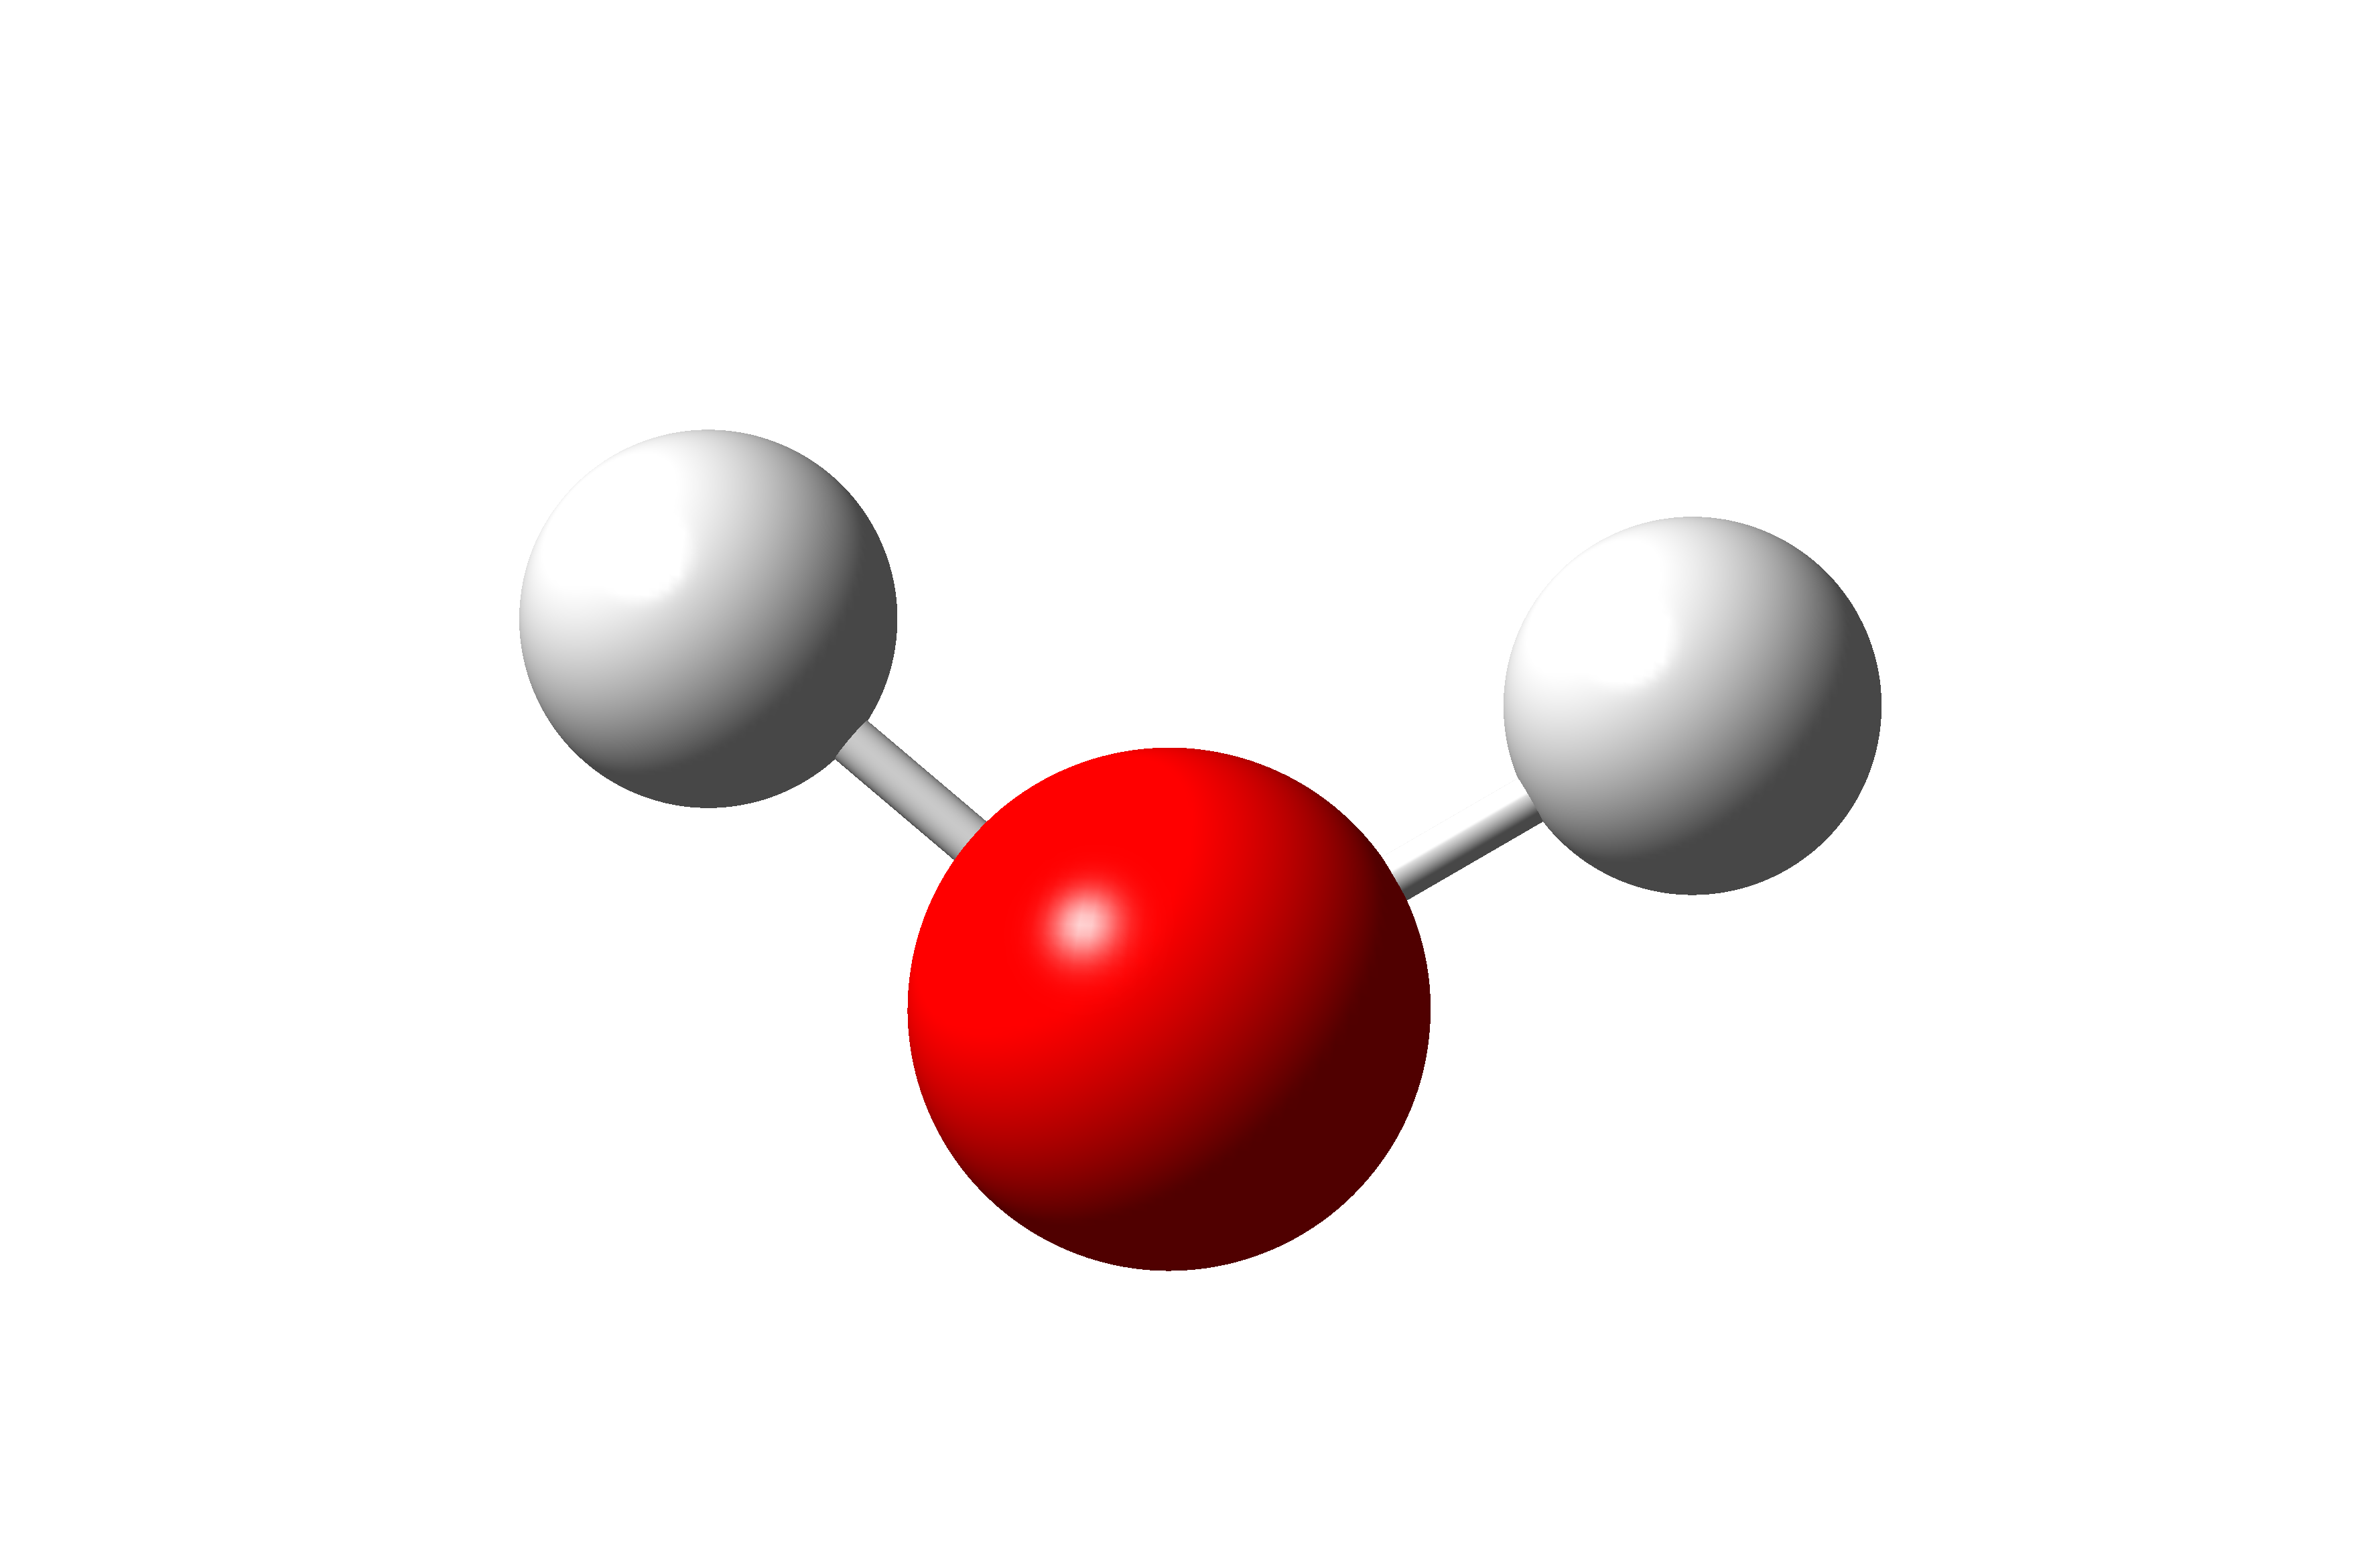
\includegraphics[width=0.2\linewidth]{../CMS/w1w.png}
\end{figure}
\begin{table}[H]
	\begin{tabular}{cccc}
		\hline
		Atom charges & Mulliken & NPA & ESP(MK) \\ \hline
		O &-0.603 & -0.936 & -0.724  \\
		H &0.302 & 0.468 & 0.362   \\
		H &0.302 & 0.468 & 0.362   \\
		\hline
	\end{tabular}
	\caption{Atomic charges (a.u.) on each atom of non-polarized water}
	\label{key}
\end{table}
All results are calculated under M06-2X/def2-QZVP with Gaussian16.
\end{frame}
\section{Polarized Water}

\begin{frame}
\frametitle{Case I}
\begin{figure}[H]
	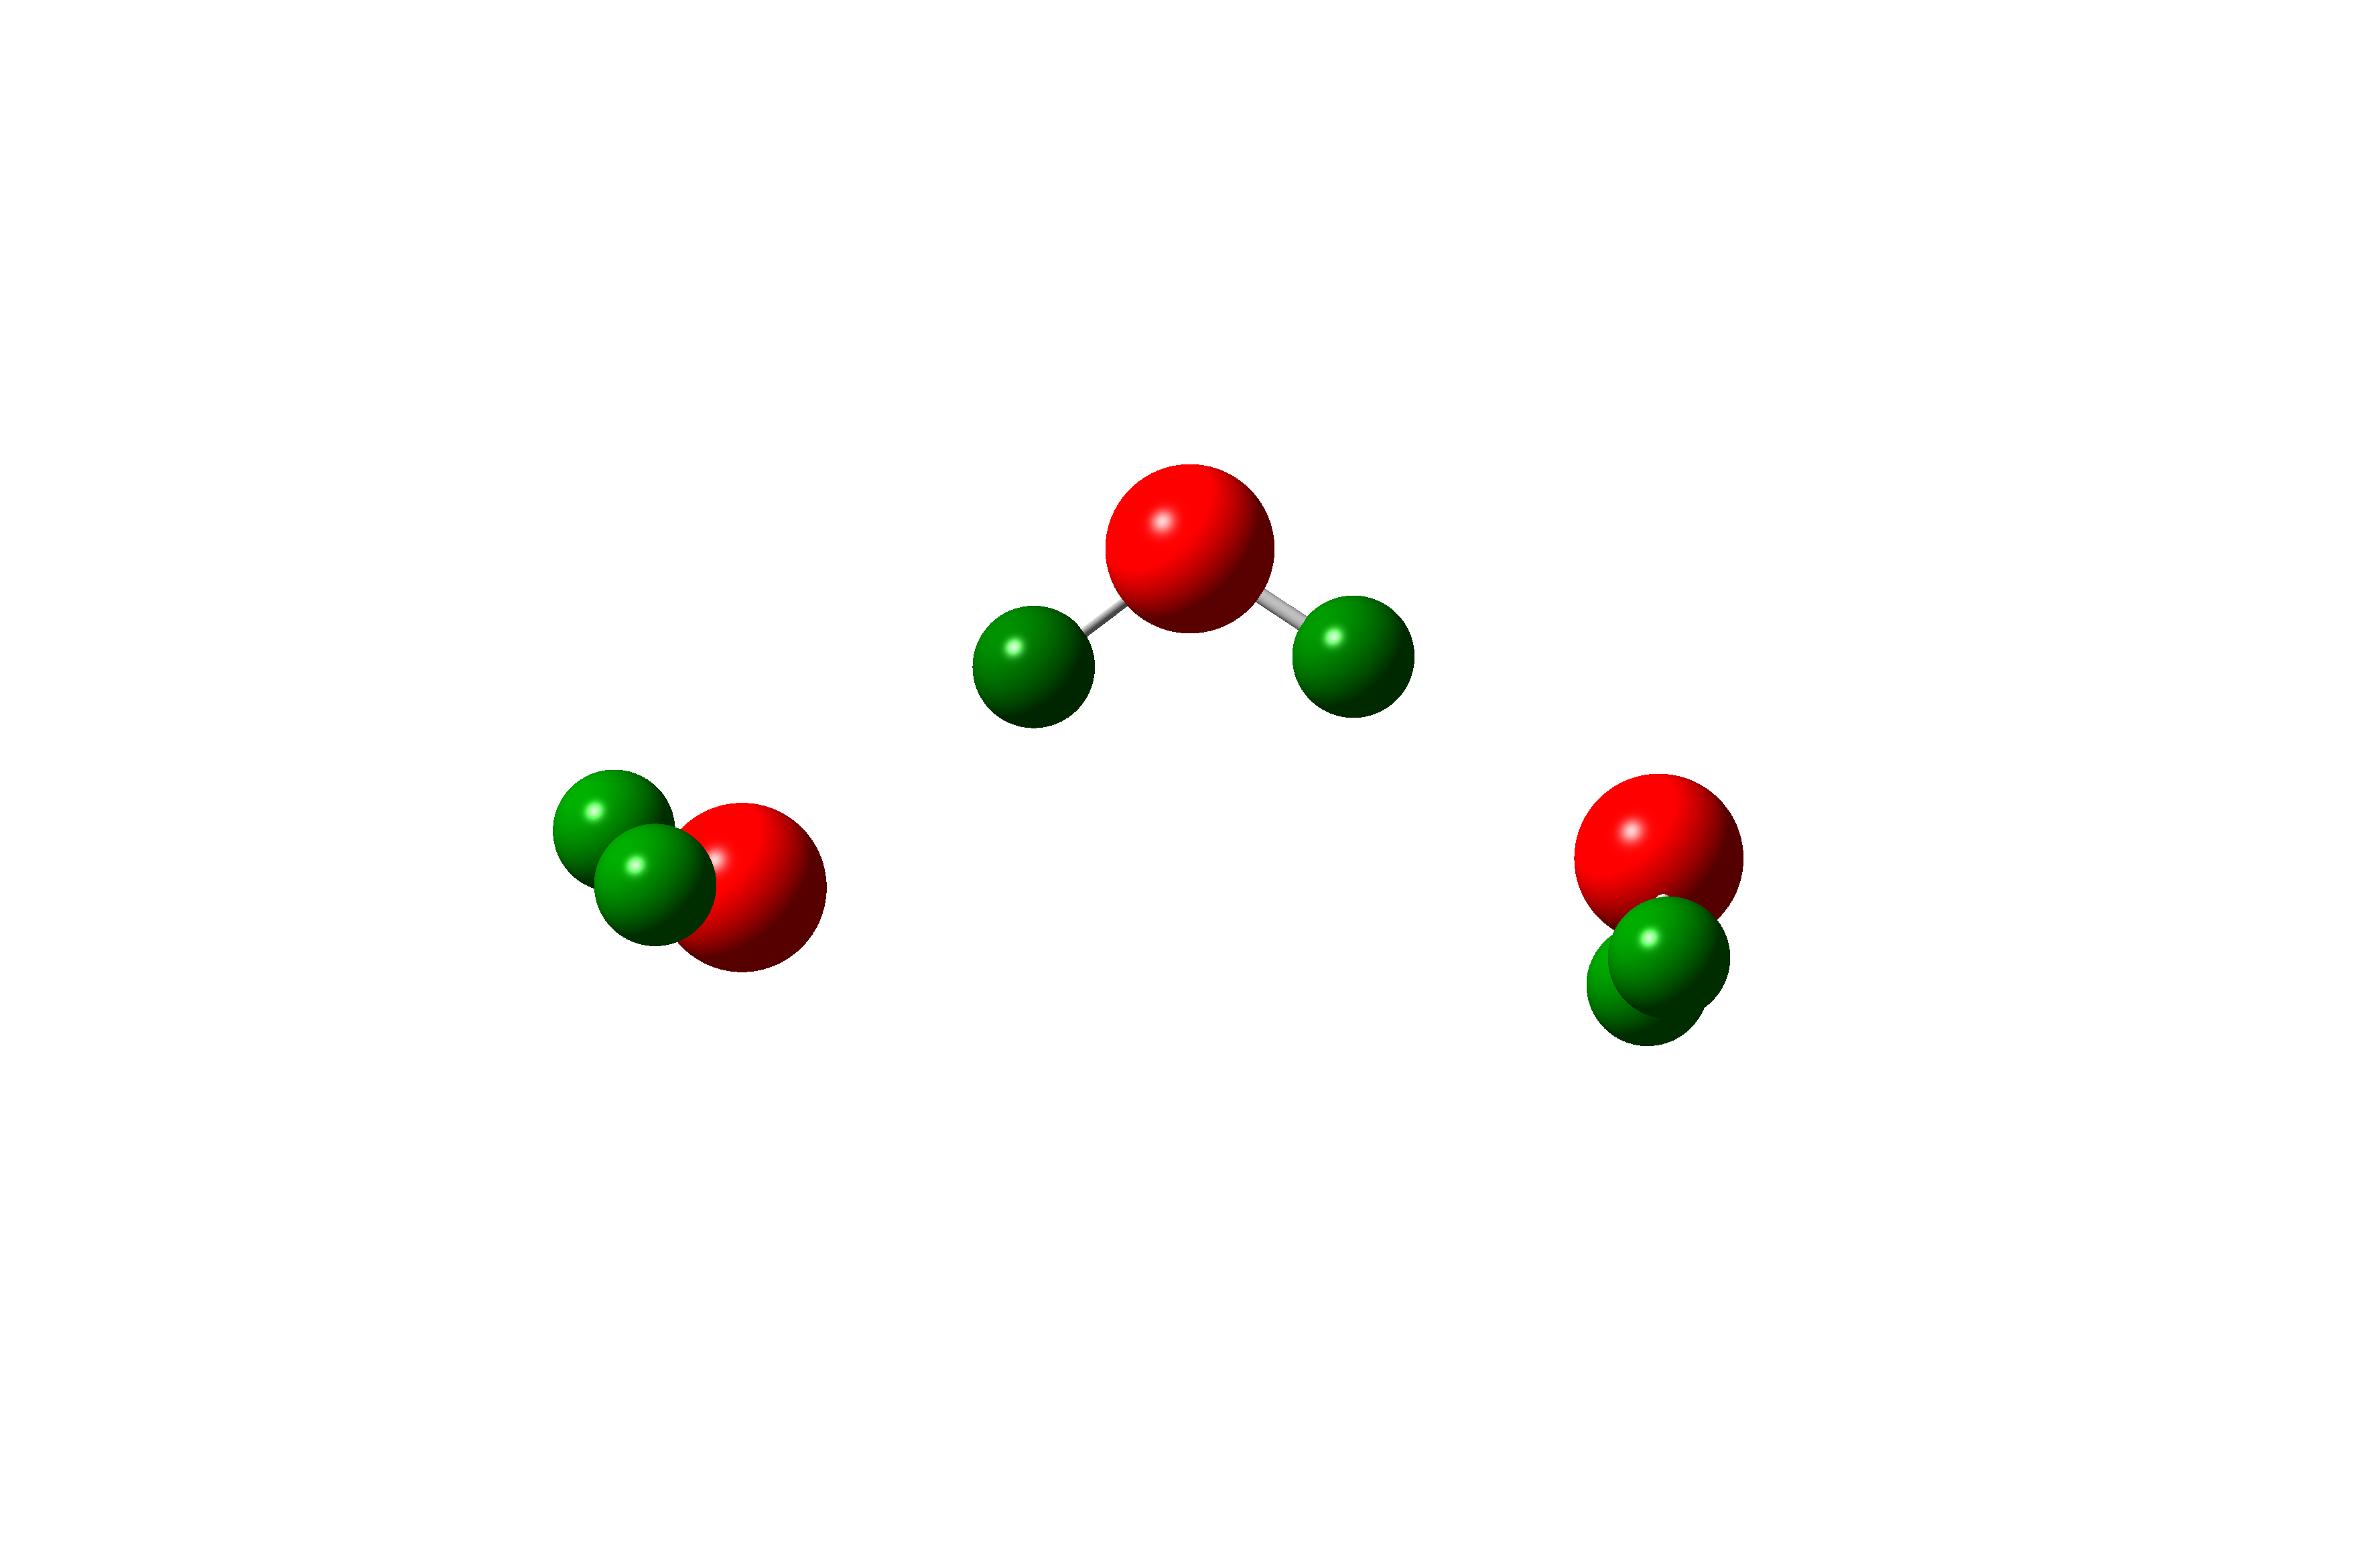
\includegraphics[width=0.4\linewidth]{../CMS/w3bwhite.png}
\end{figure}
\begin{table}[H]
	\begin{tabular}{cccc}
		\hline
		Atom charges & Mulliken & NPA & ESP(MK) \\ \hline
		O &-0.642 & -1.011 & -0.877  \\
		H &0.295 & 0.486 & 0.449   \\
		H &0.274 & 0.483 & 0.379   \\
		\hline
	\end{tabular}
	\caption{Atomic charges (a.u.) on each atom of polarized water, Case I}
	\label{key}
\end{table}
\end{frame}

\begin{frame}
\frametitle{Case II}
\begin{figure}[H]
	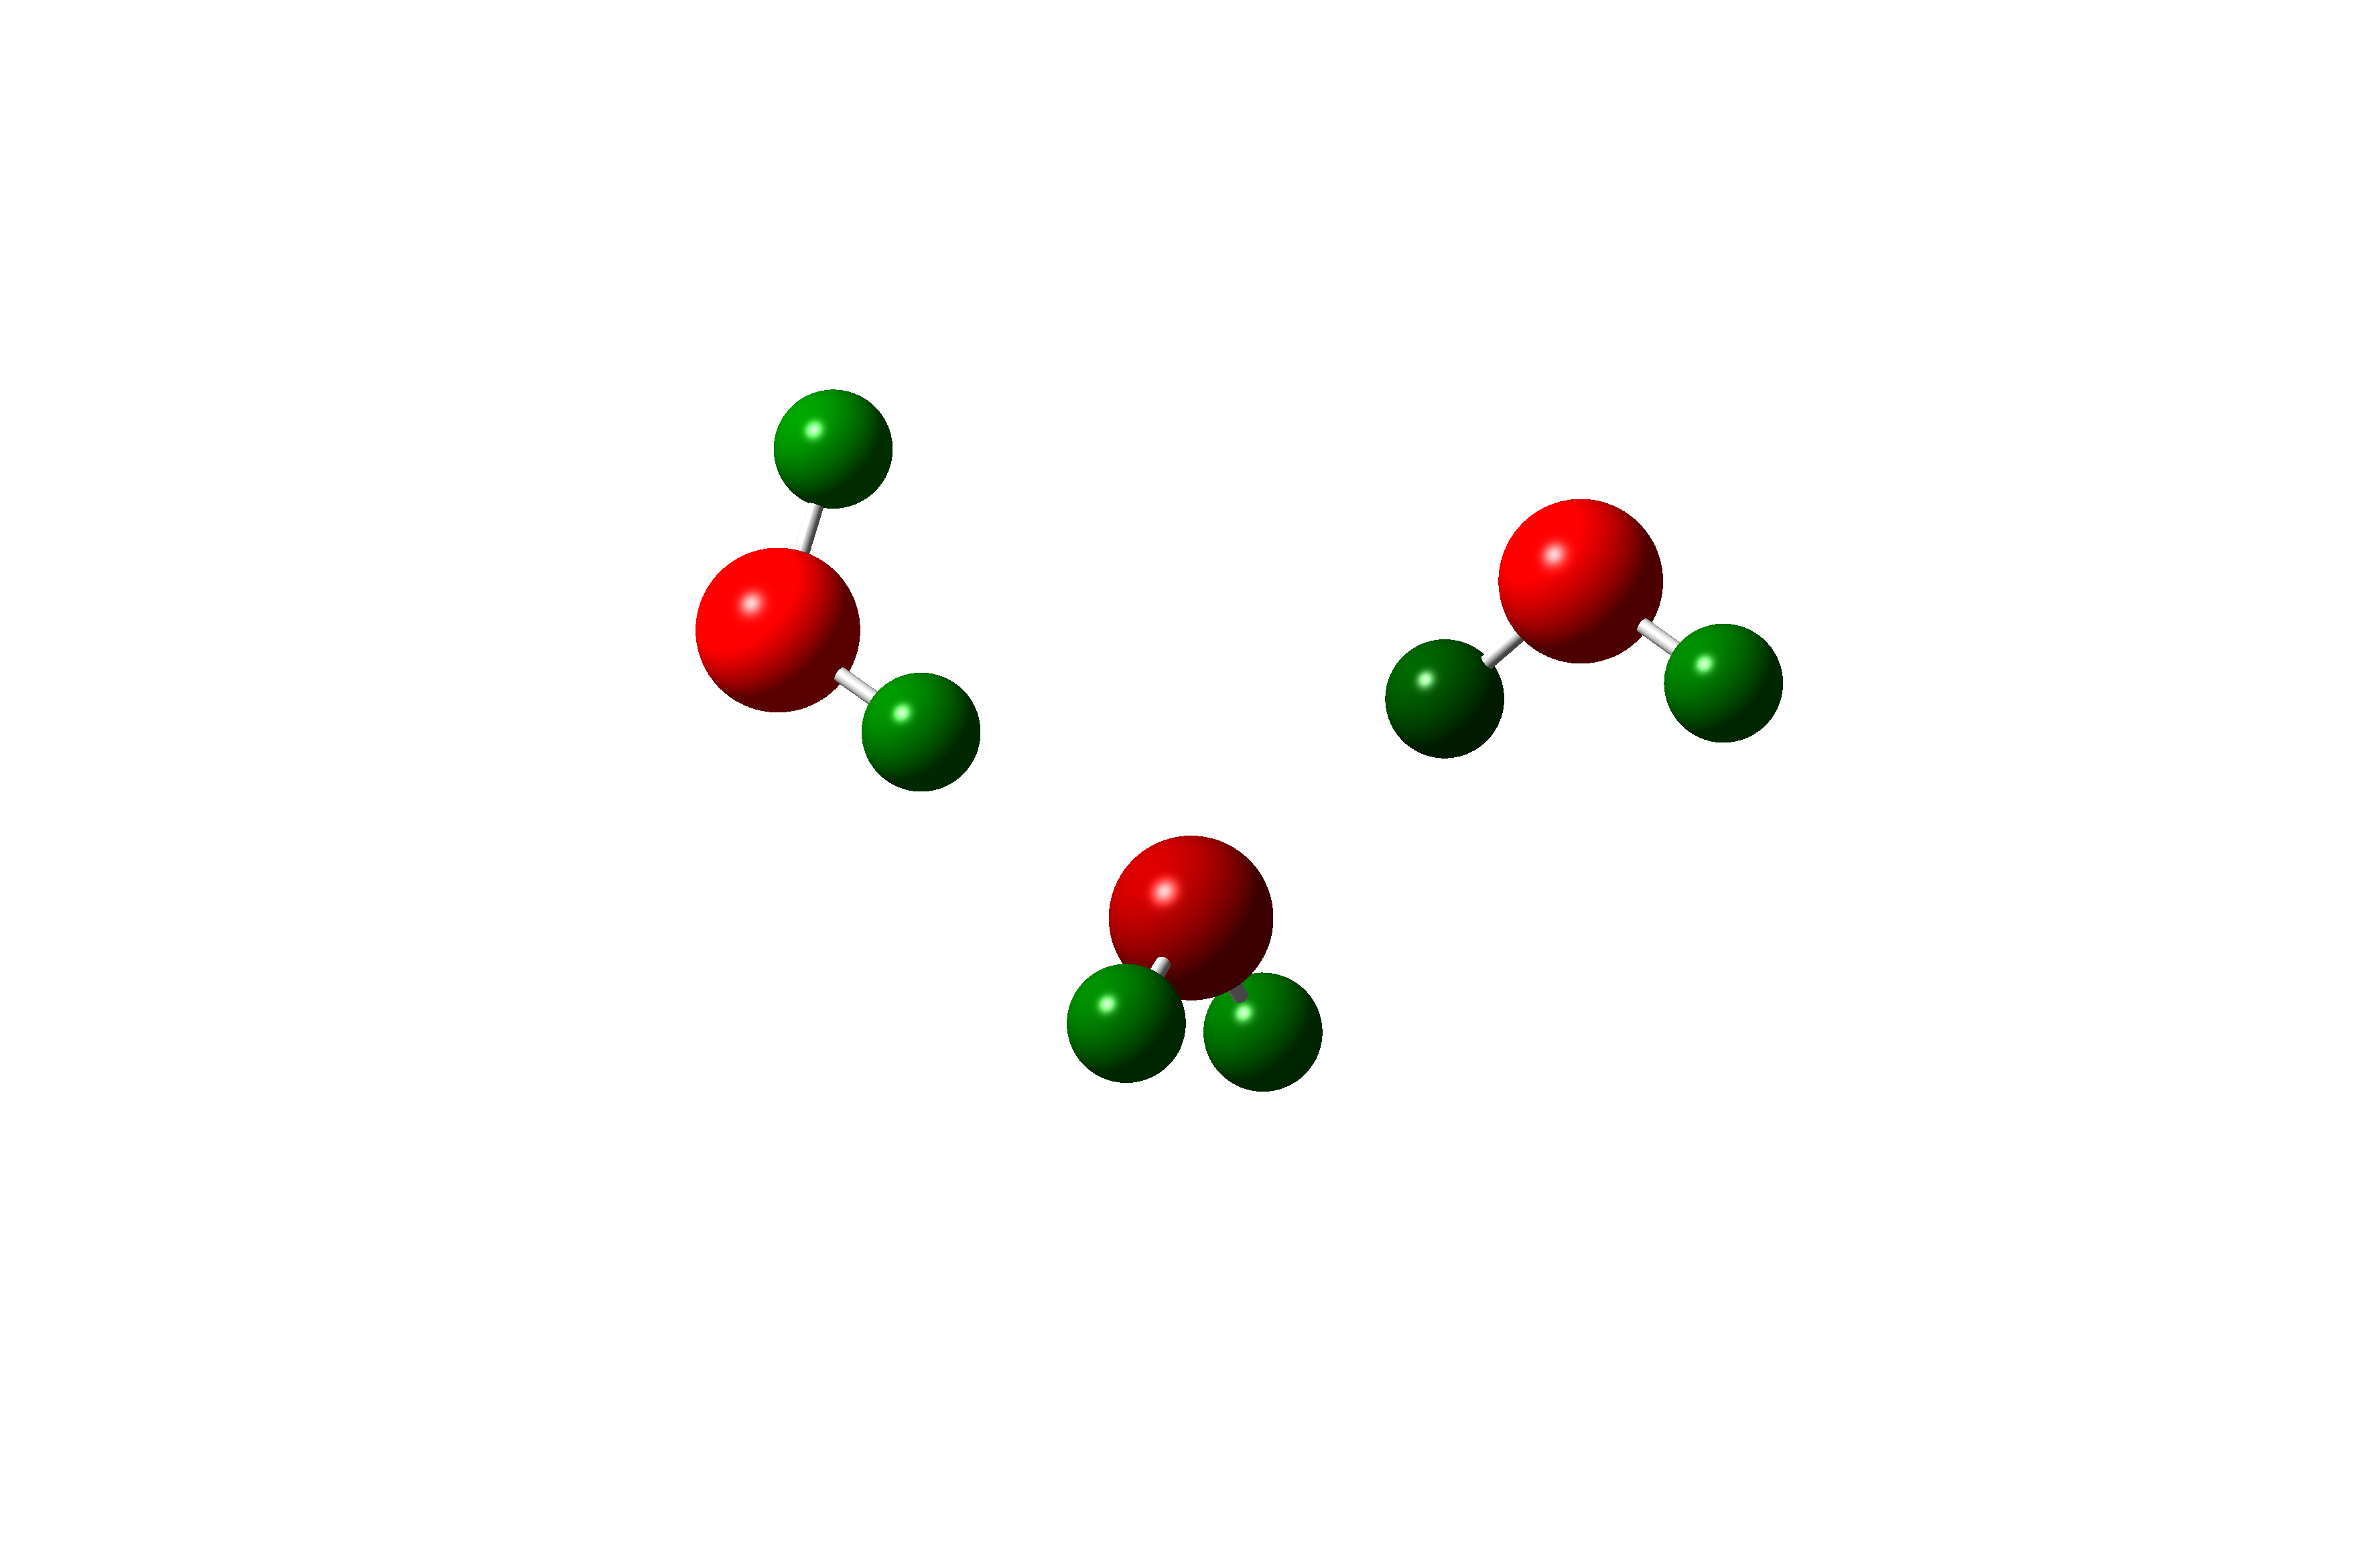
\includegraphics[width=0.4\linewidth]{../CMS/w3cw.png}
\end{figure}
\begin{table}[H]
	\begin{tabular}{cccc}
		\hline
		Atom charges & Mulliken & NPA & ESP(MK) \\ \hline
		O &-0.655 & -0.950 & -0.550  \\
		H &0.353 & 0.496 & 0.358   \\
		H &0.352 & 0.495 & 0.341   \\
		\hline
	\end{tabular}
	\caption{Atomic charges (a.u.) on each atom of polarized water, Case II}
\end{table}
\end{frame}

\begin{frame}
\frametitle{Case III -- with Background Charges}
\begin{figure}[H]
	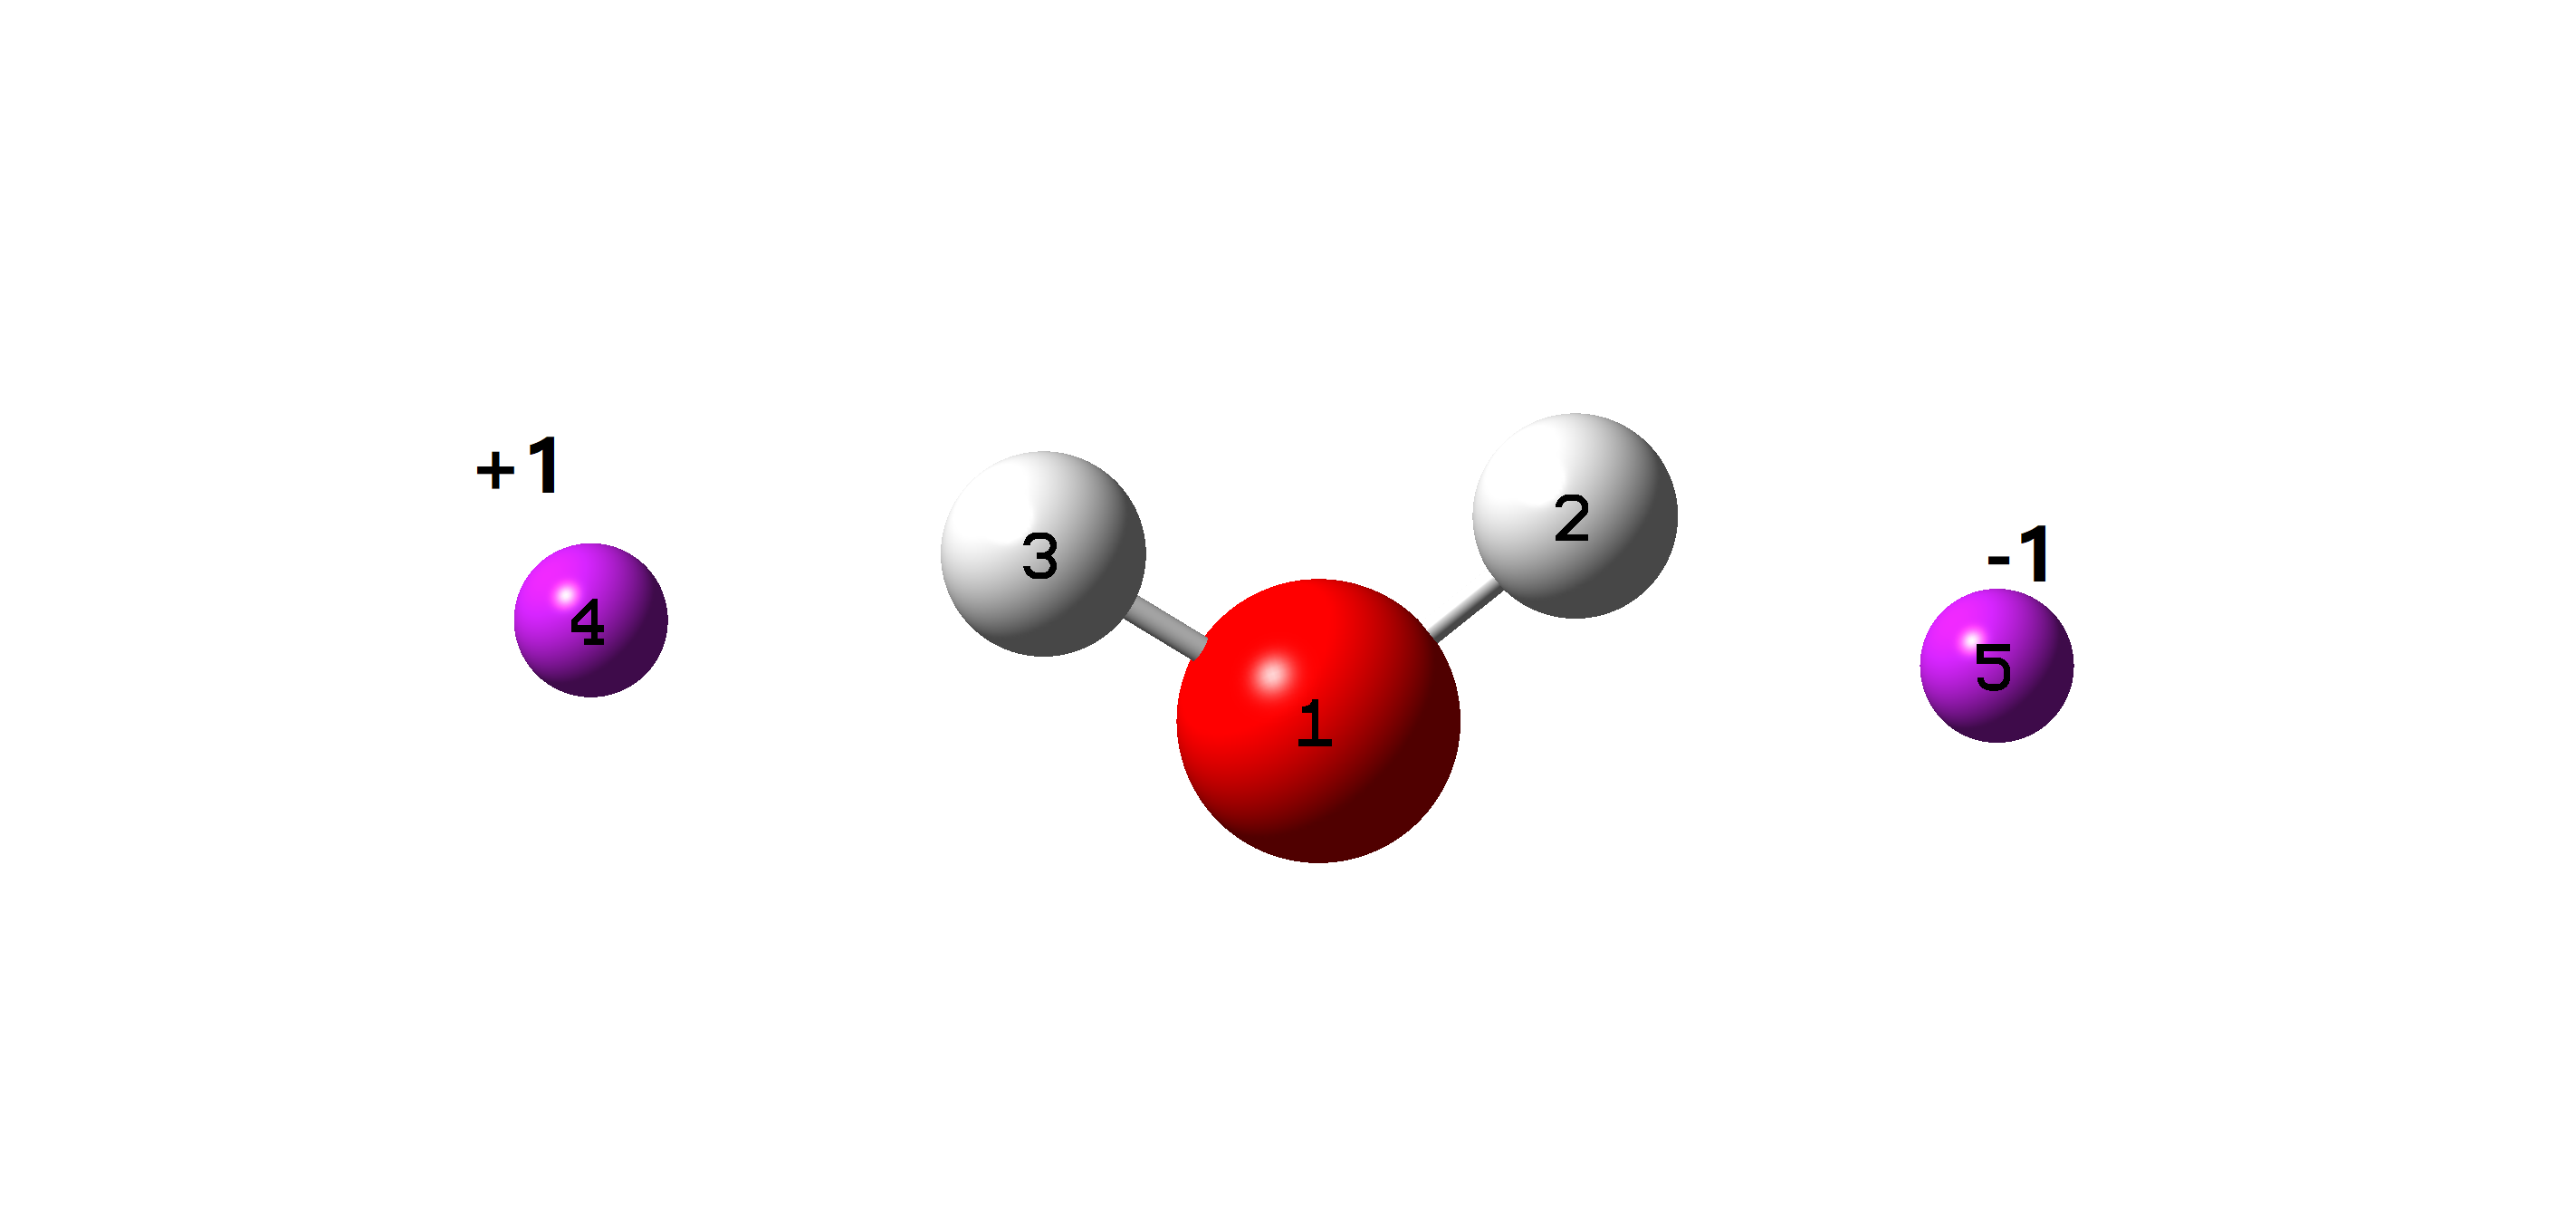
\includegraphics[width=0.6\linewidth]{../CMS/w1bqw.png}
\end{figure}
\begin{table}[H]
	\begin{tabular}{cccc}
		\hline
		Atom charges & Mulliken & NPA & ESP(MK) \\ \hline
		O & -0.365 & -0.787 & -0.523  \\
		H & 0.720 & 0.647 & 0.725  \\
		H & -0.354 & 0.139 & -0.202   \\
		\hline
	\end{tabular}
	\caption{Atomic charges (a.u.) on each atom of polarized water, Case III}
\end{table}
\end{frame}



\section{Solvated Water}
\begin{frame}
\frametitle{Case IV -- Solvated Water}
%\vspace{-10pt}
%\begin{figure}[H]
%	%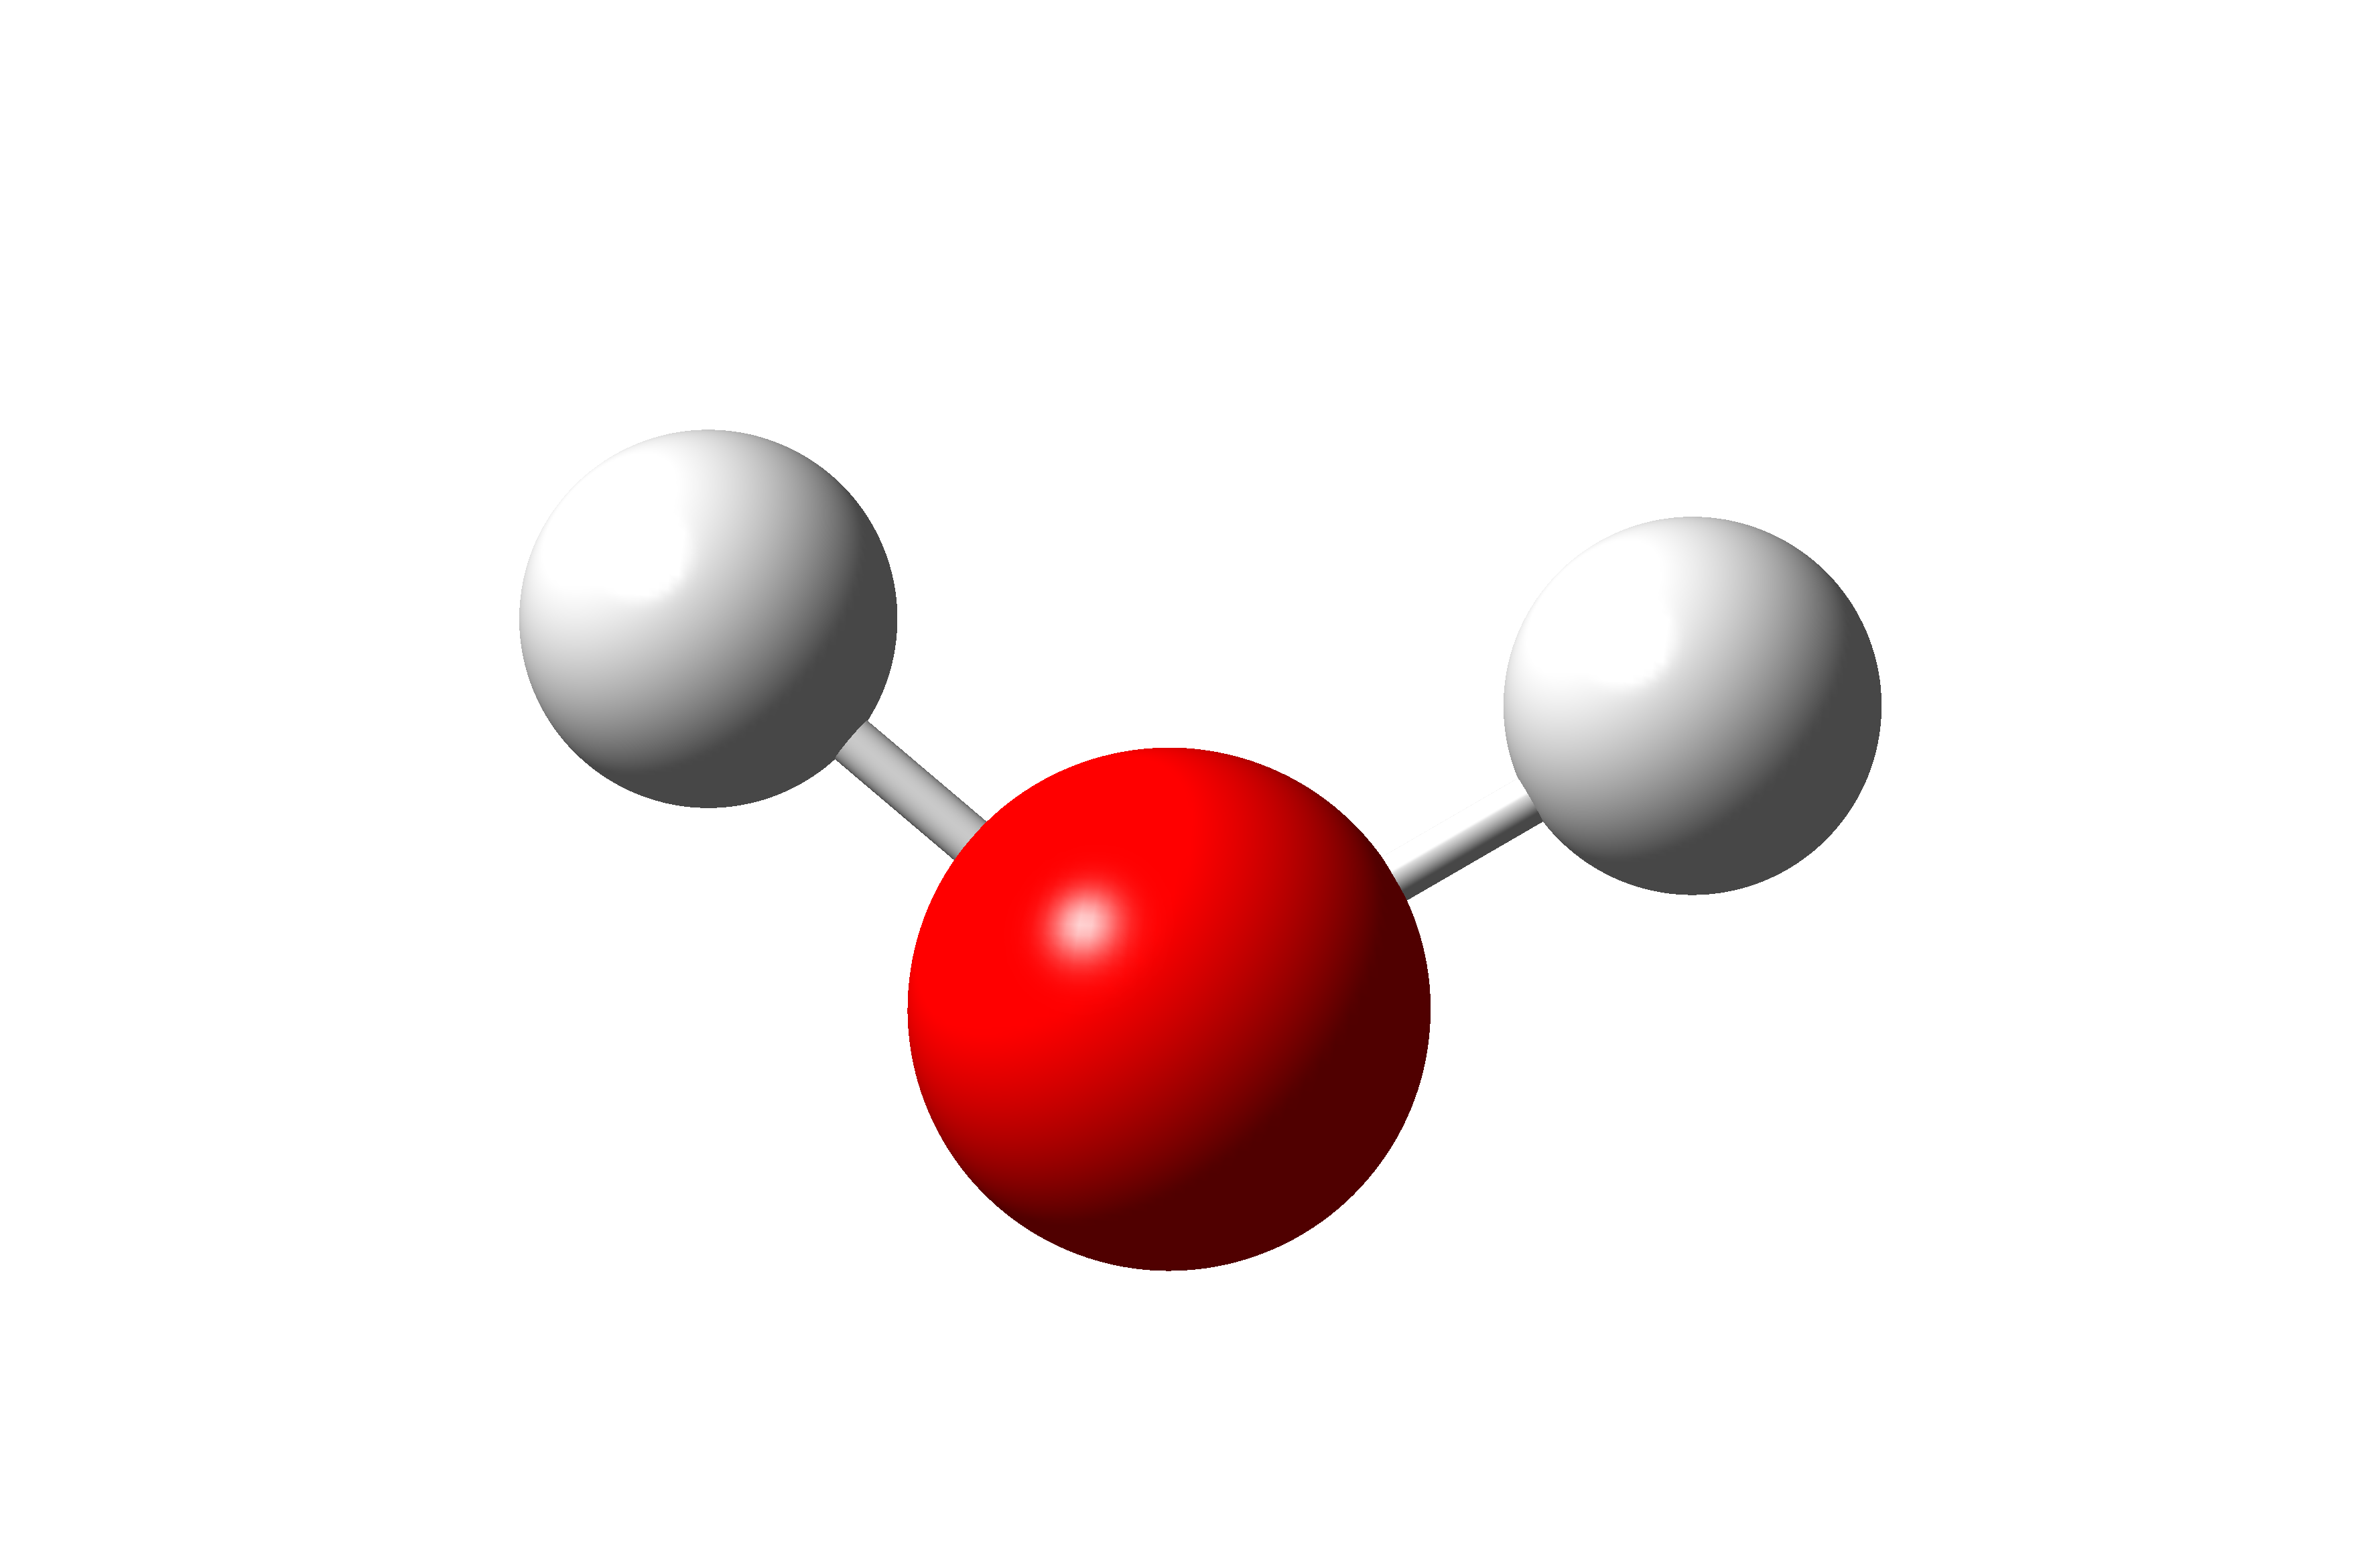
\includegraphics[width=0.1\linewidth]{../CMS/w1w.png}%
%	%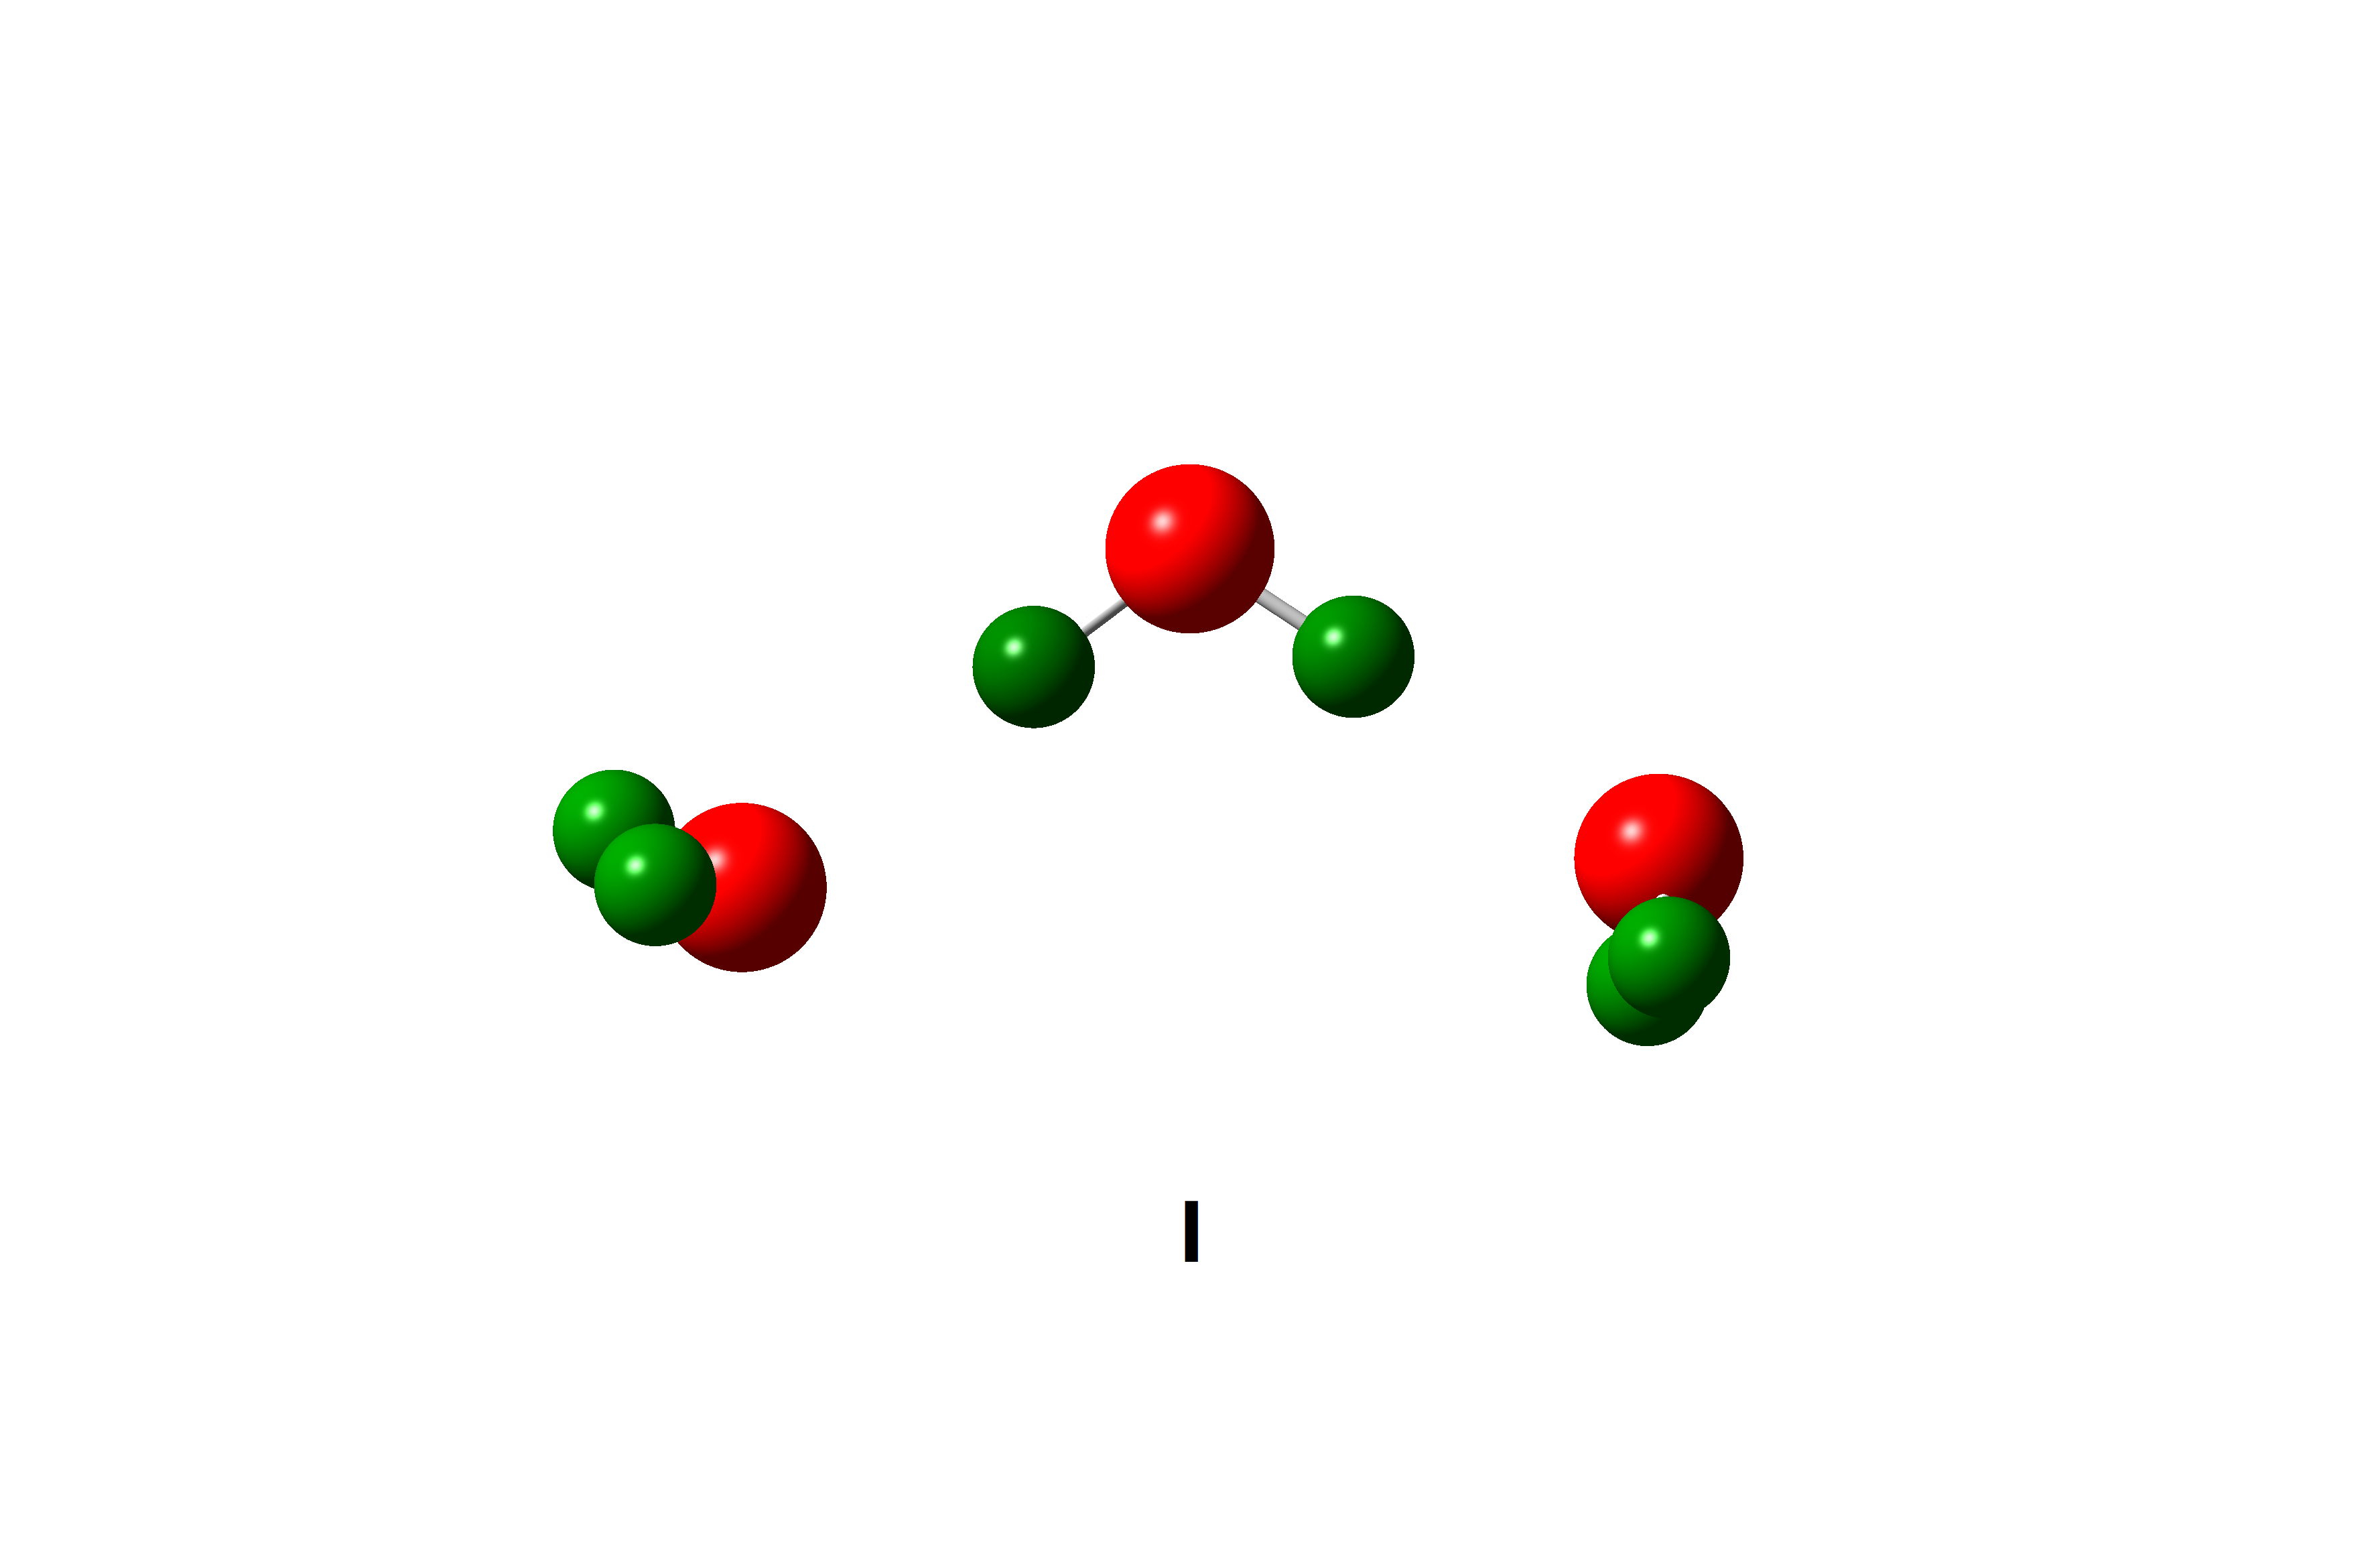
\includegraphics[width=0.4\linewidth]{../CMS/w3bw2.png}
%	%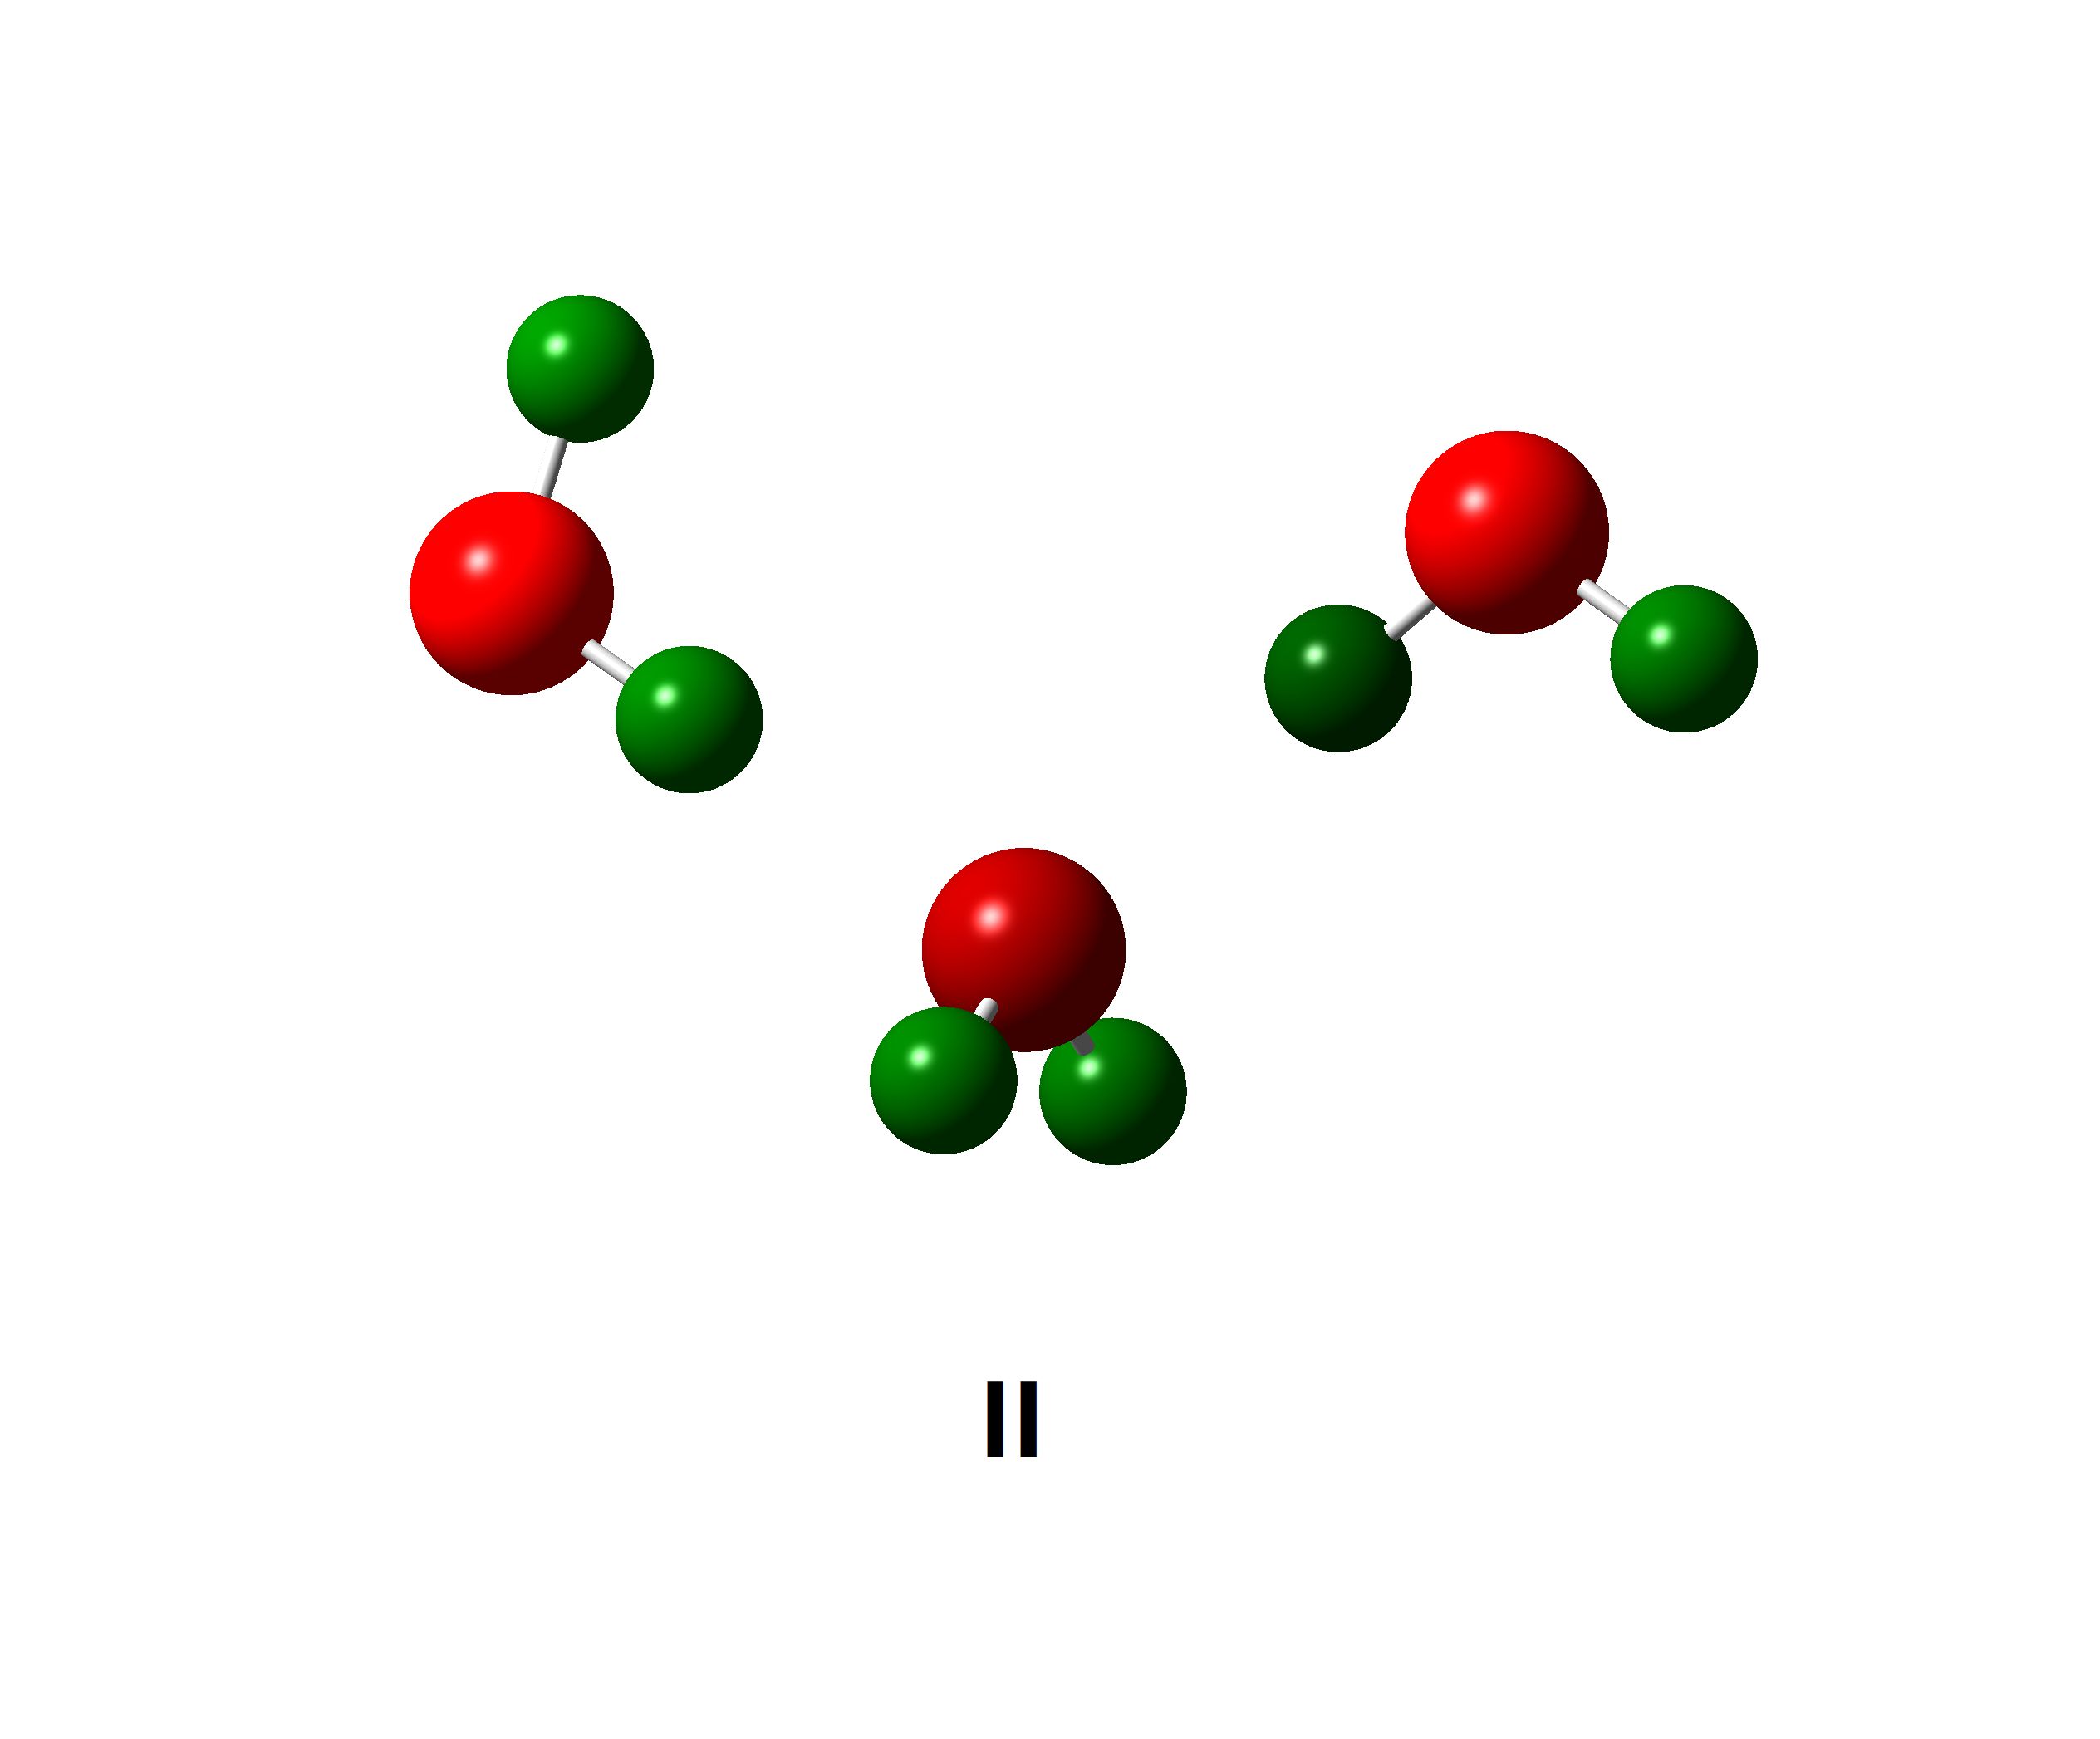
\includegraphics[width=0.3\linewidth]{../CMS/w3cw2.png}
%	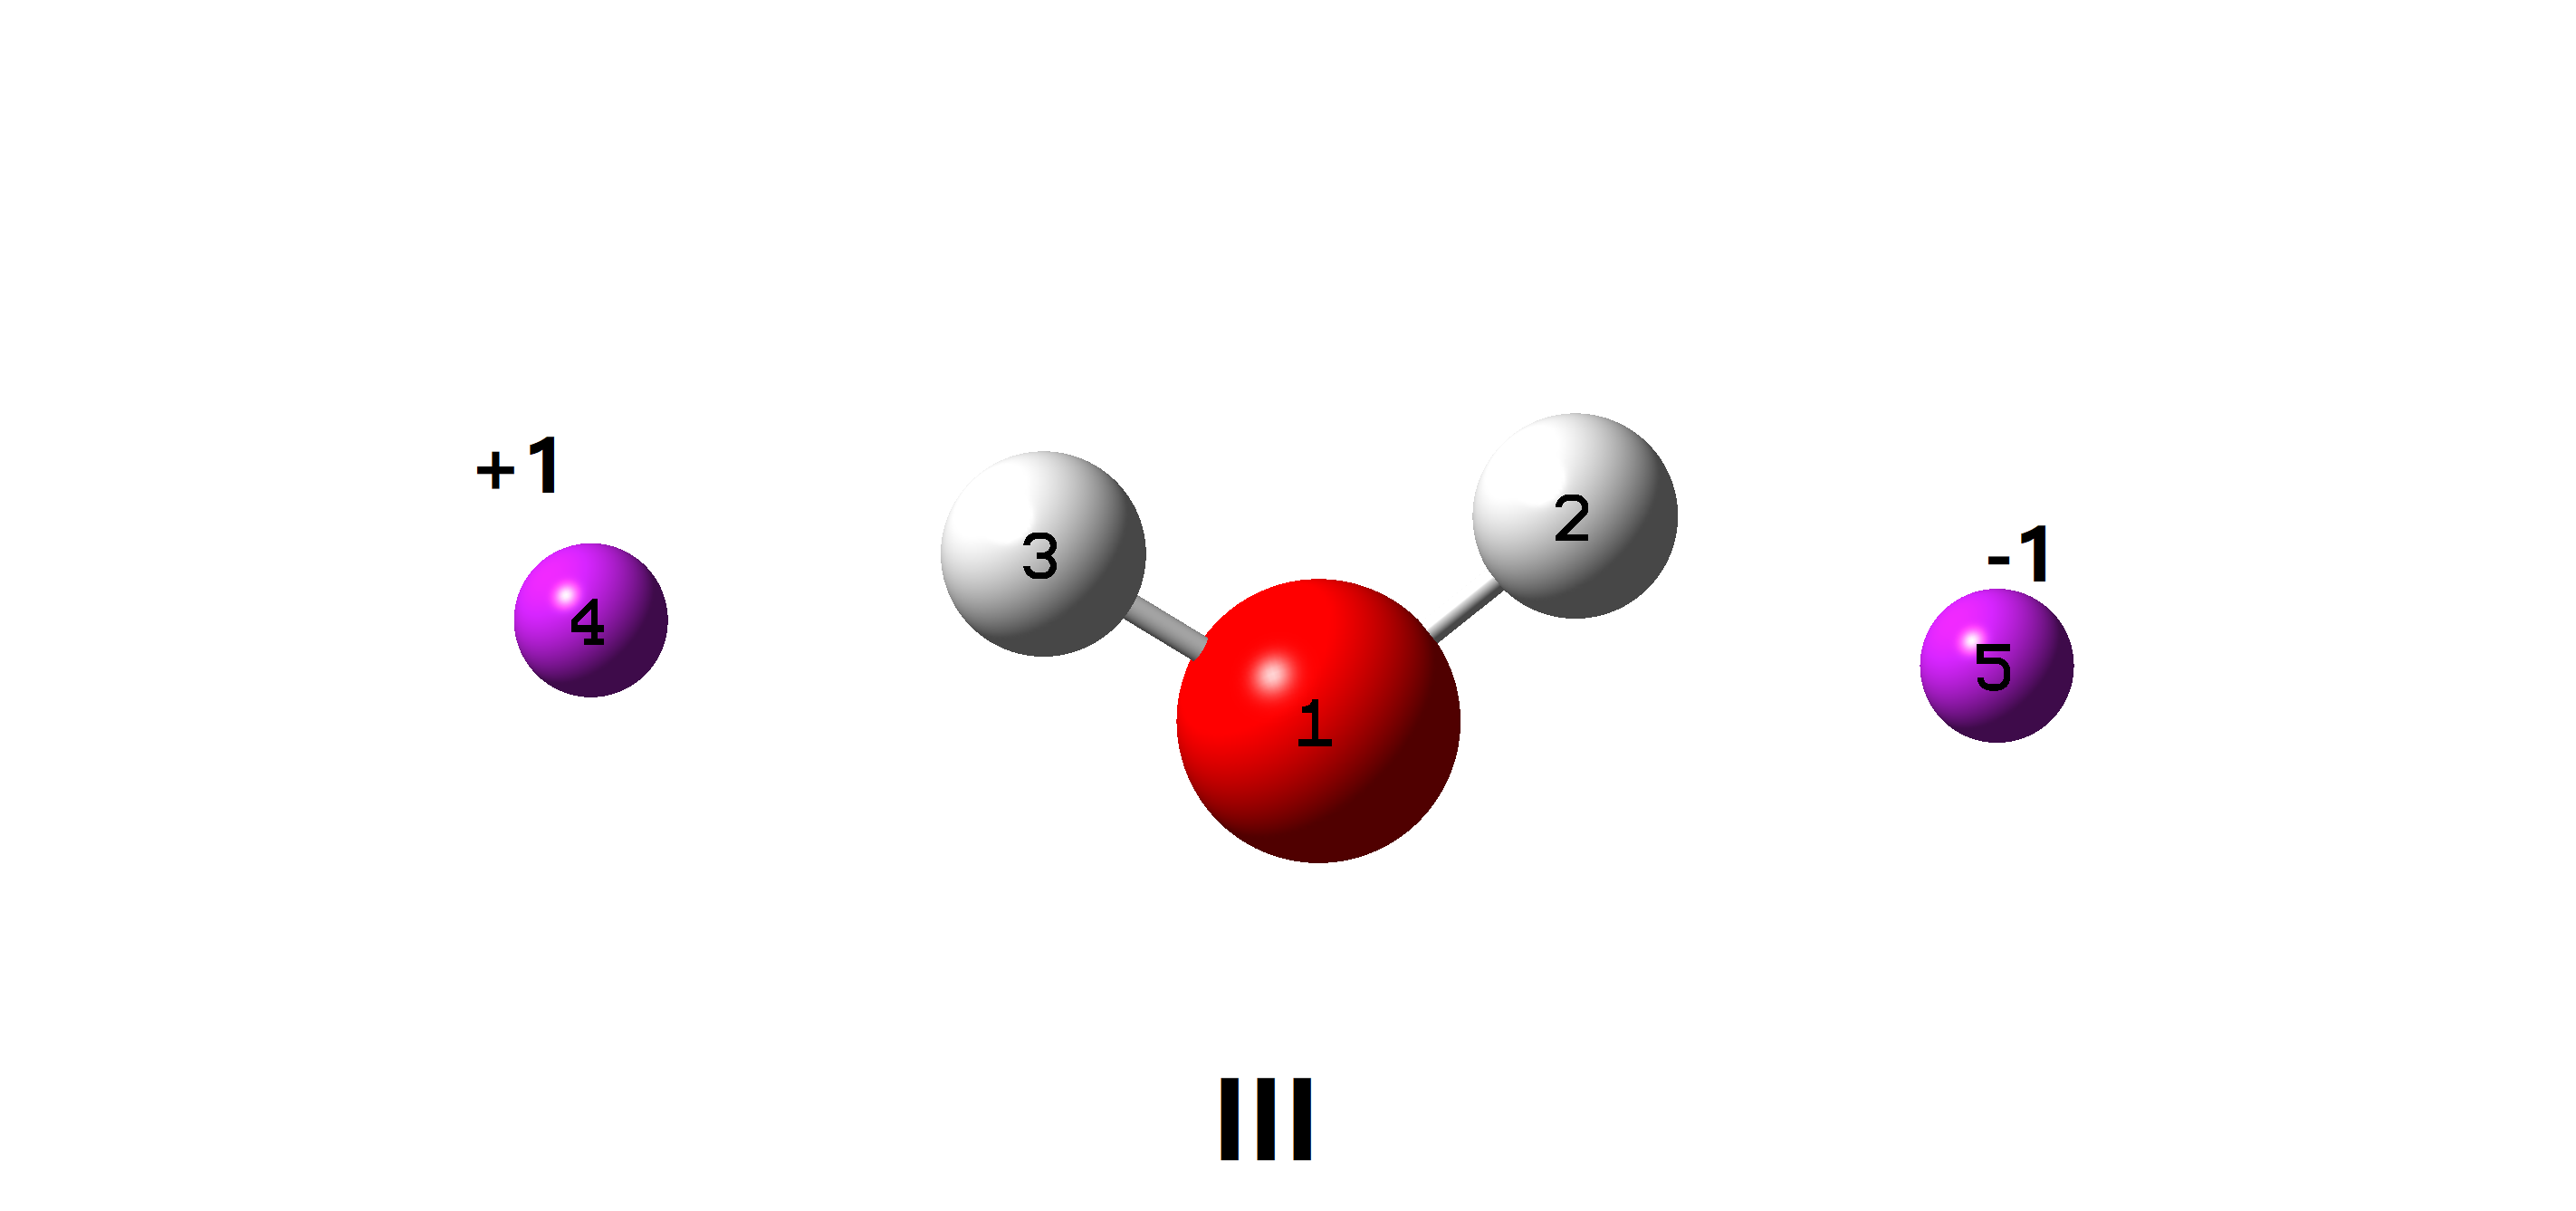
\includegraphics[width=0.35\linewidth]{../CMS/w1bqw2.png}
%\end{figure}
\begin{table}[H]
	\begin{tabular}{cccc}
		\hline
		Atom charges & Mulliken & NPA & ESP(MK) \\ \hline
		O & -0.640 & -0.950 & -0.763  \\
		H & 0.320 & 0.475 & 0.381  \\
		H & 0.320 & 0.475 & 0.381   \\
		\hline
	\end{tabular}
	\caption{Atomic charges (a.u.) on each atom of water in cyclohexane solvent (PCM model)}
\end{table}
The results show that water molecule is a little bit more polarized in cyclohexane.
\end{frame}

\section{Summary}
\begin{frame}
\frametitle{Summary}
\vspace{-10pt}
\begin{figure}[H]
	%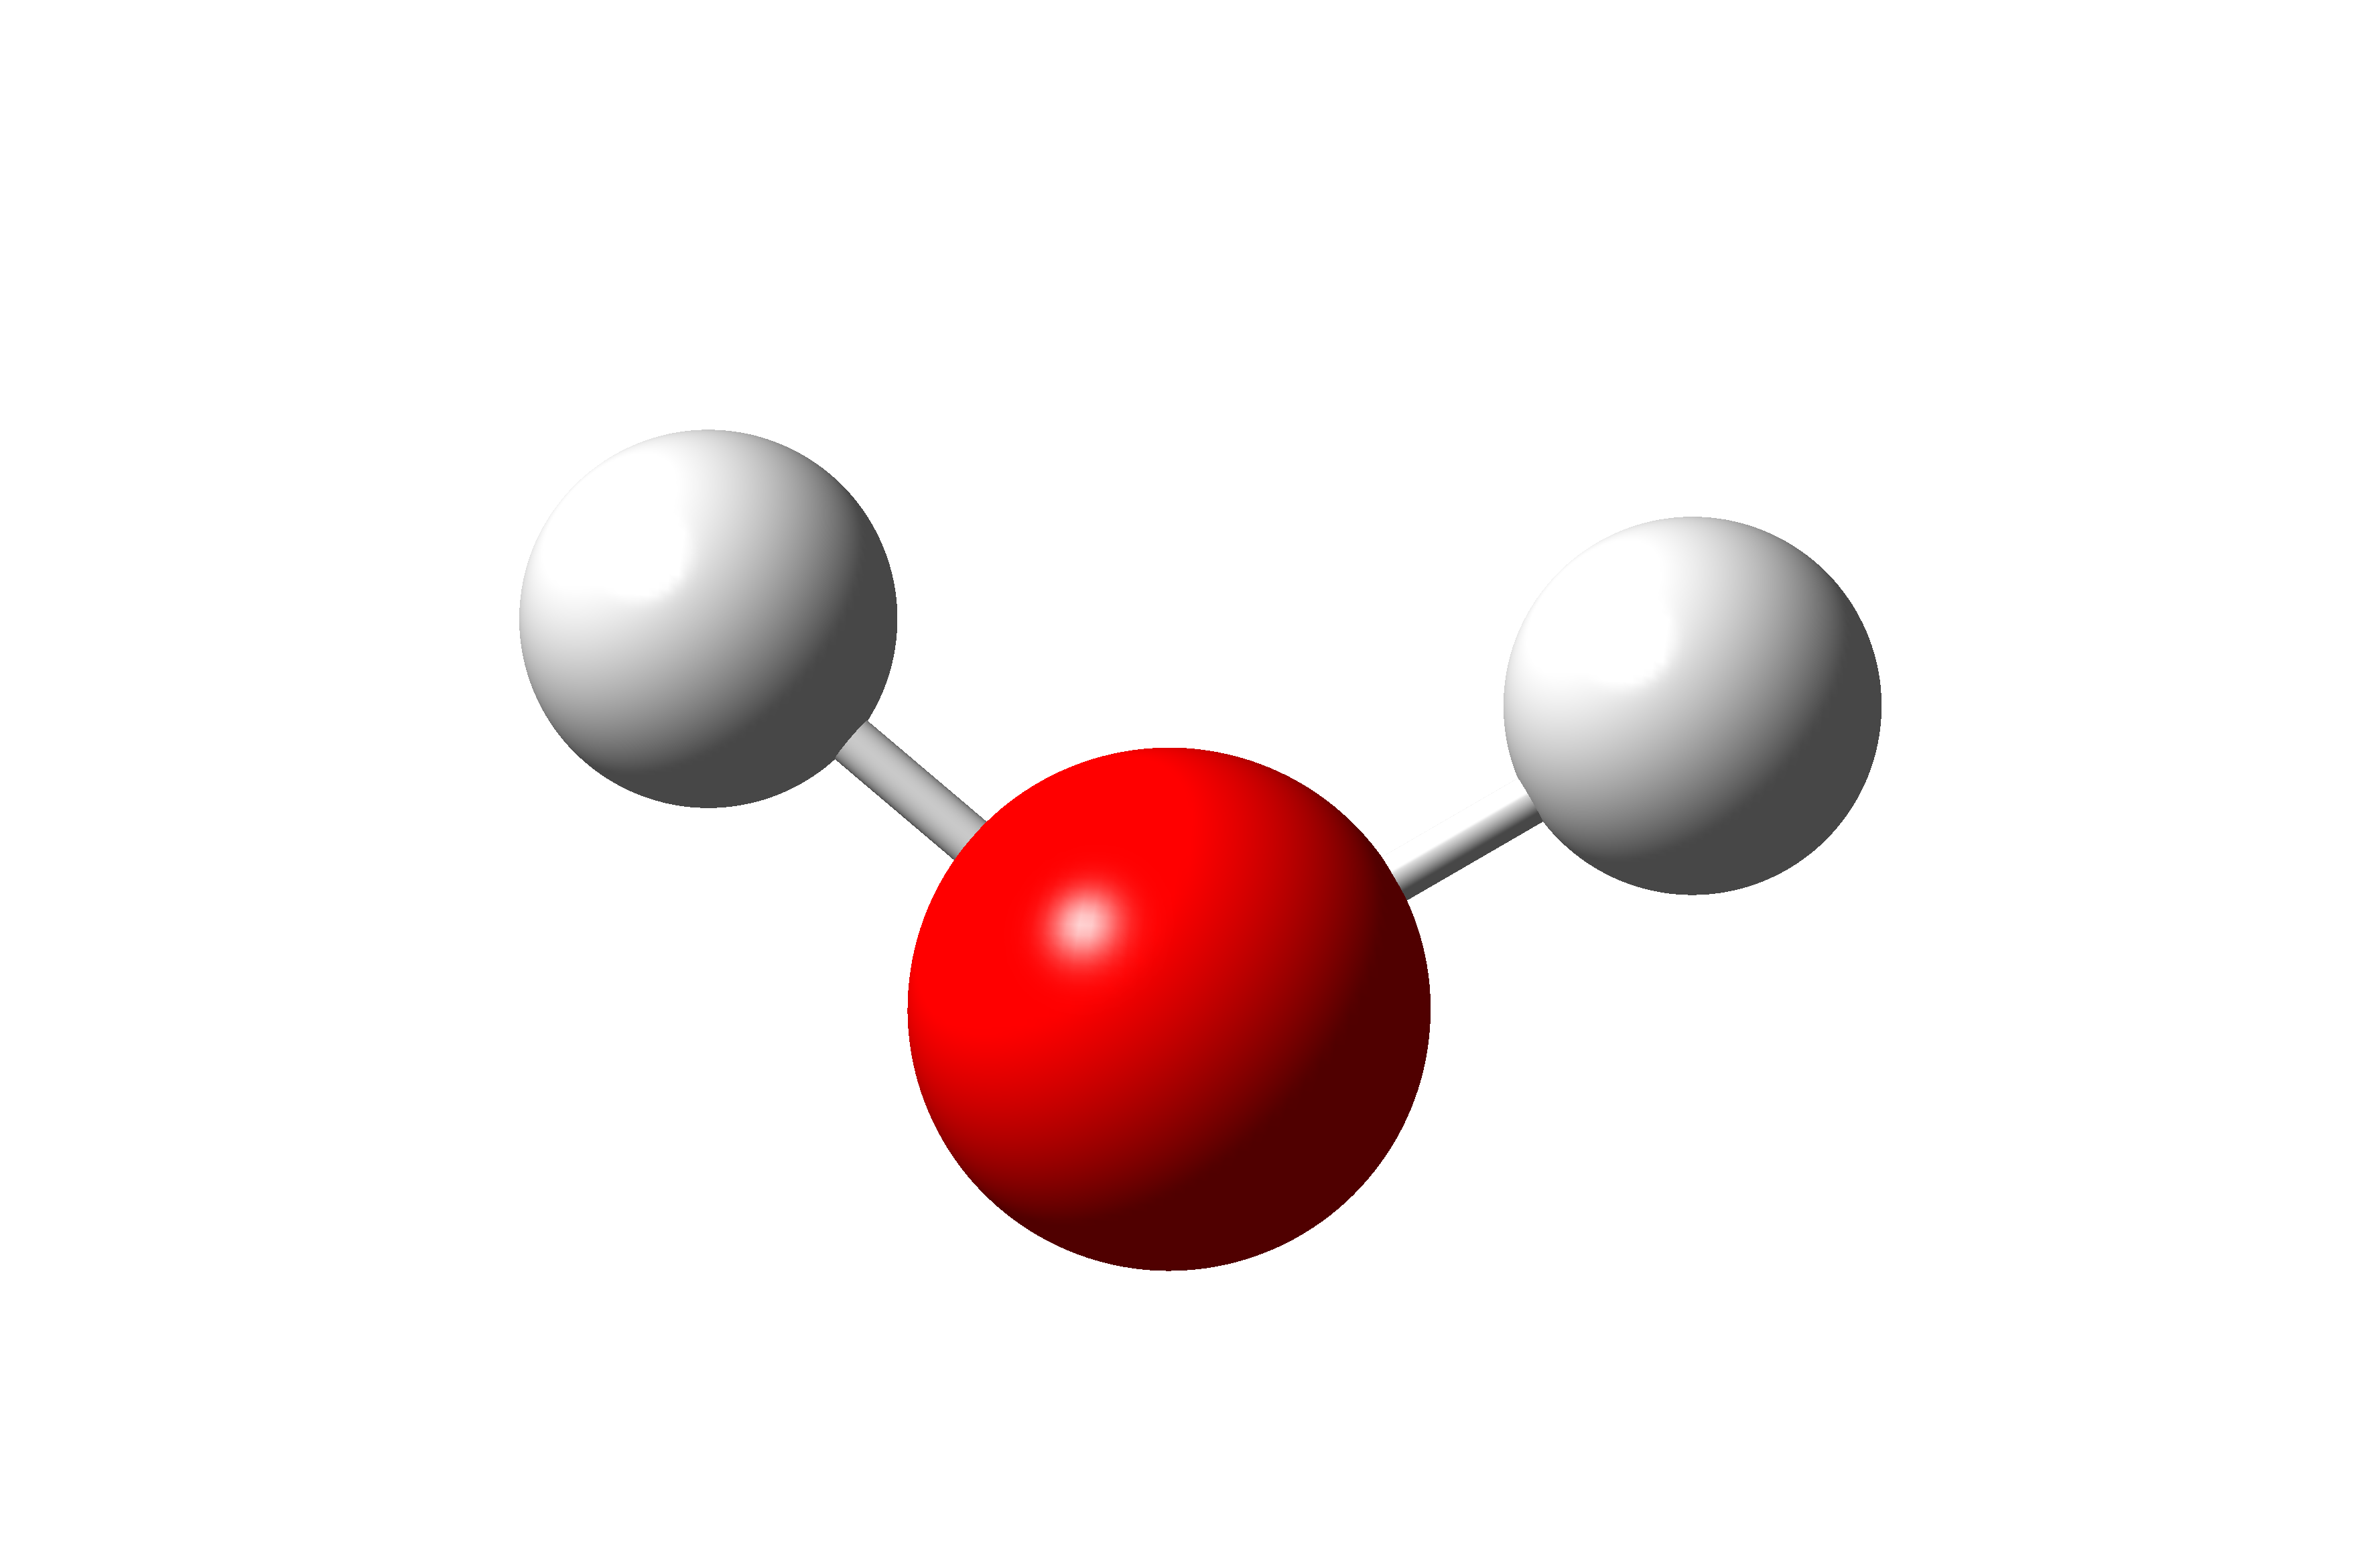
\includegraphics[width=0.1\linewidth]{../CMS/w1w.png}
	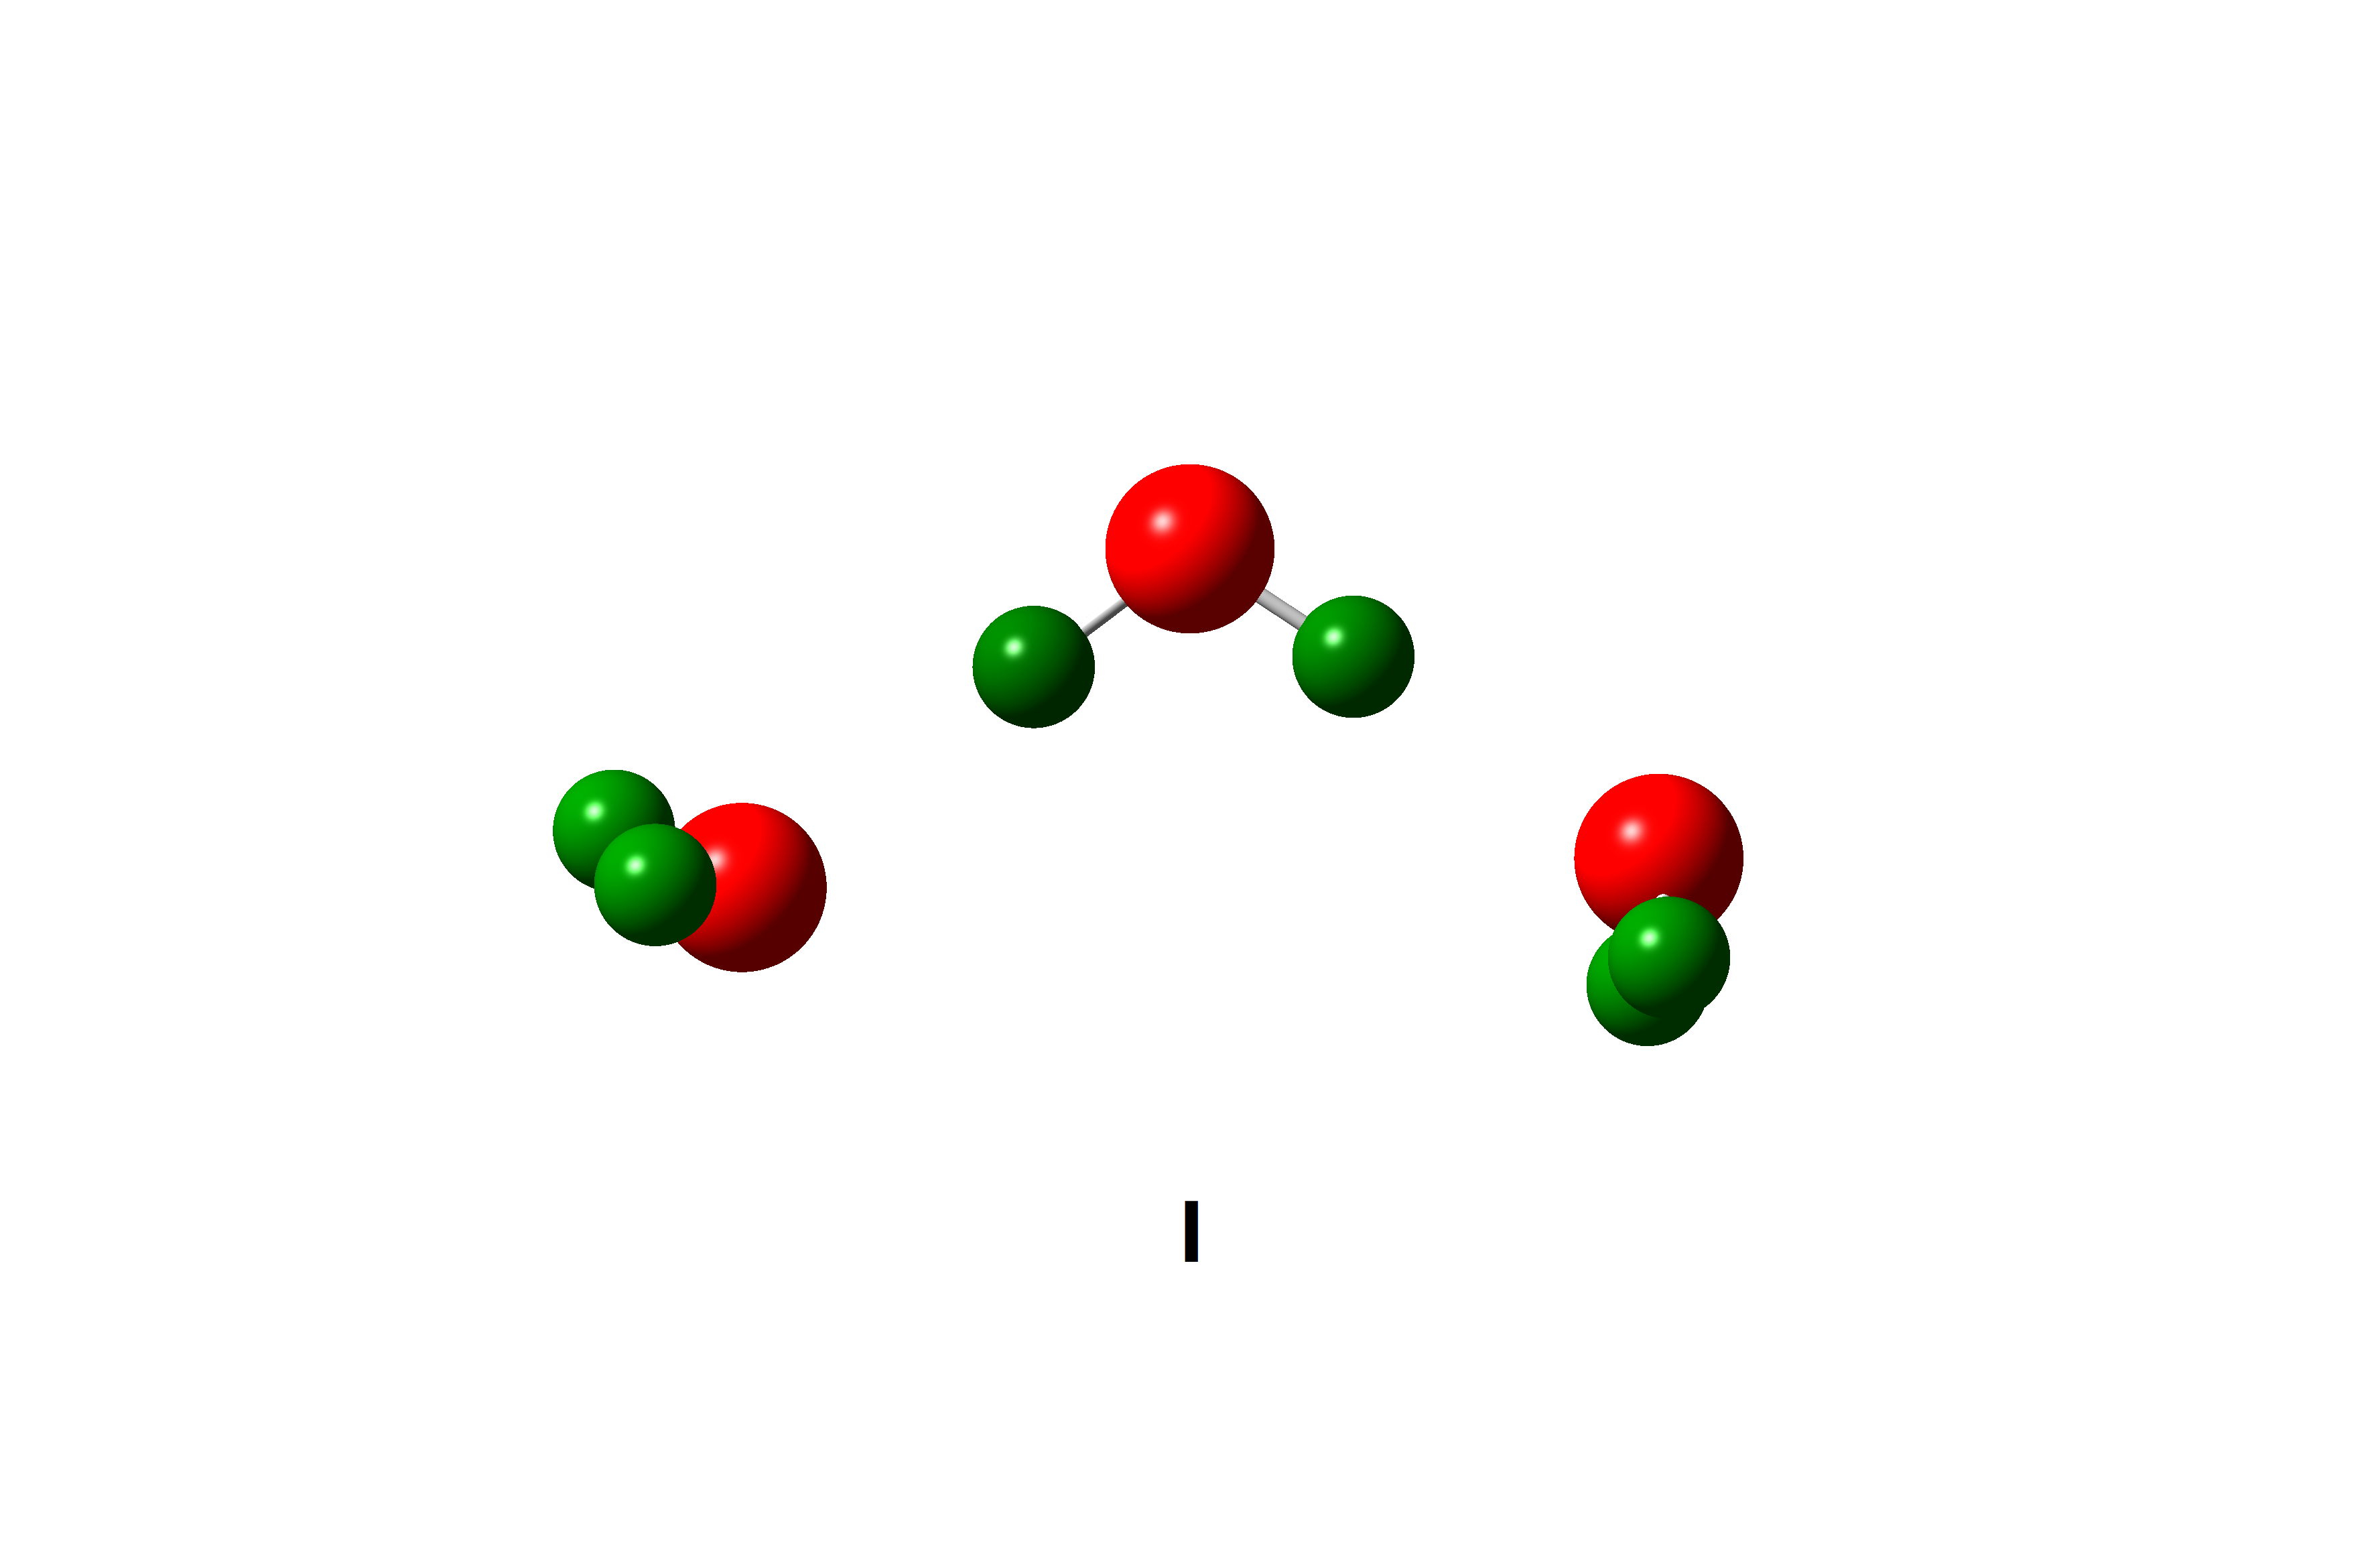
\includegraphics[width=0.4\linewidth]{../CMS/w3bw2.png}
	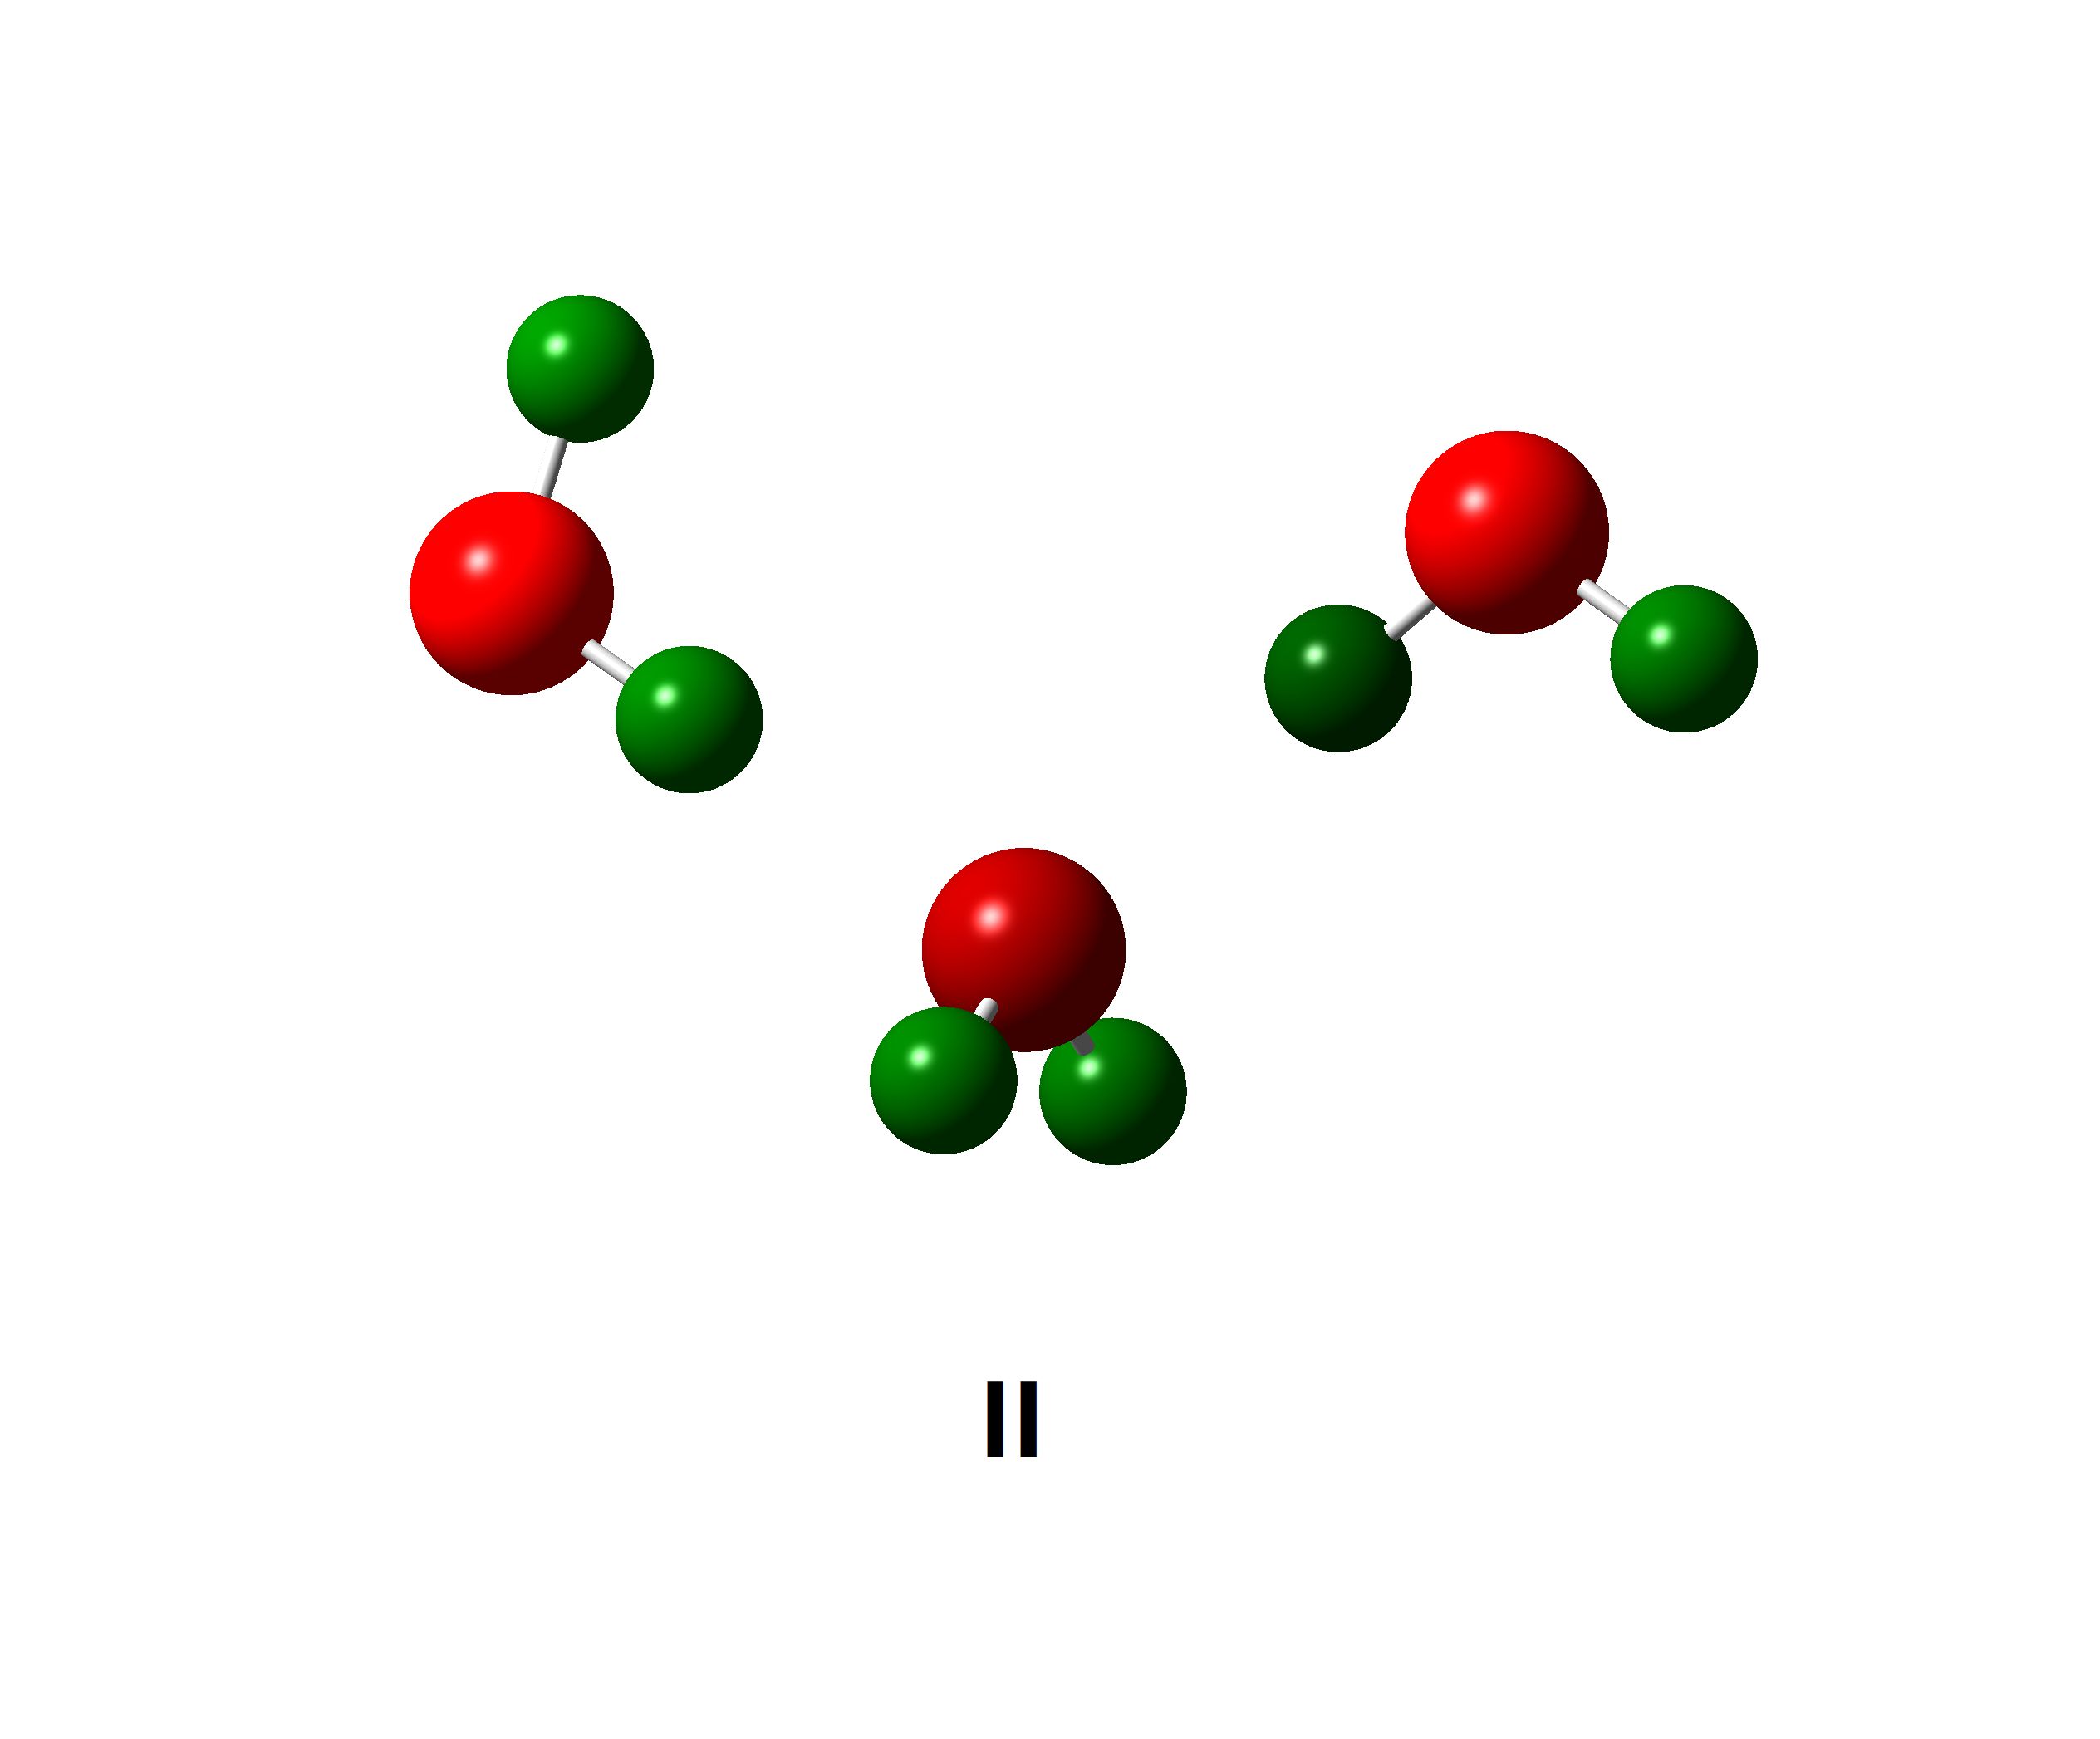
\includegraphics[width=0.3\linewidth]{../CMS/w3cw2.png}
	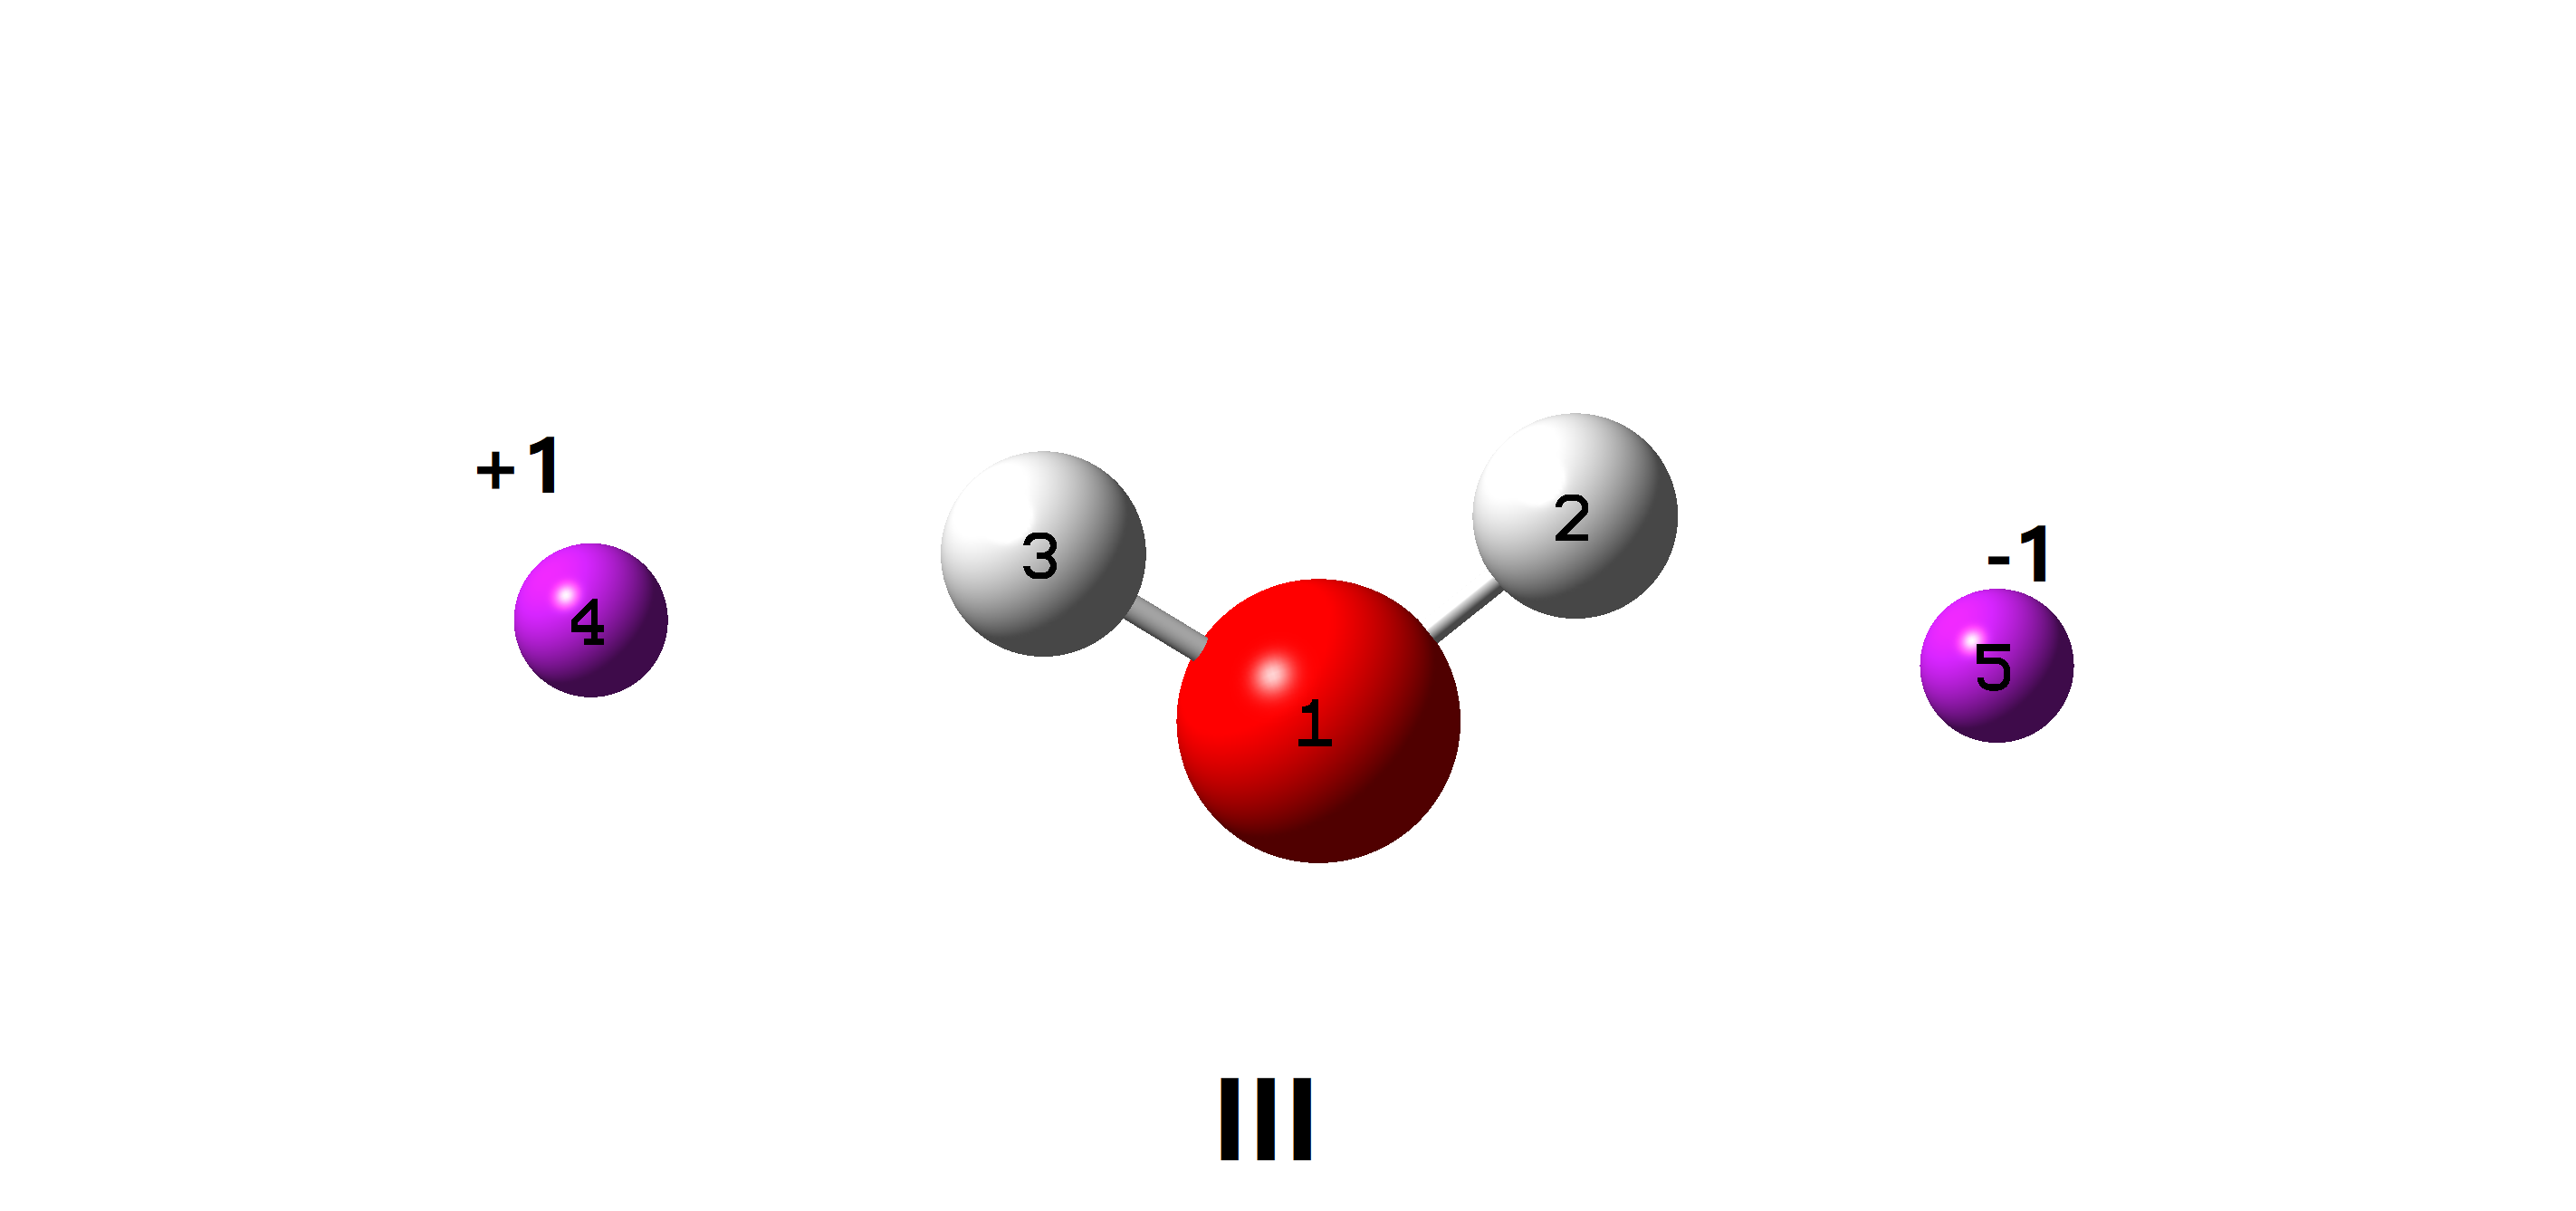
\includegraphics[width=0.35\linewidth]{../CMS/w1bqw2.png}
\end{figure}
\begin{table}[H]
	\begin{tabular}{cccccc}
		\hline
		Atom & non-polarized & I & II & III & IV\\ \hline
		O &0	&-0.153	&0.174	&0.201  & -0.039\\
		H &0	&0.087	&-0.004	&0.363  & 0.019\\
		H &0	&0.017	&-0.021	&-0.564 & 0.019\\		
		\hline
	\end{tabular}
	\caption{changes of ESP charges on each atom (set non-polarized results as zero)}
\end{table}
\end{frame}


\begin{frame}
  \begin{center}
    \Huge{\texttt{\textbf{Thank You}}}\\[0.5cm]
    %Q\&A
  \end{center}
\end{frame}


\end{document}
